%%%%%%%%%%%%%%%%%%%%%%% file template.tex %%%%%%%%%%%%%%%%%%%%%%%%%
%
% This is a general template file for the LaTeX package SVJour3
% for Springer journals.          Springer Heidelberg 2010/09/16
%
% Copy it to a new file with a new name and use it as the basis
% for your article. Delete % signs as needed.
%
% This template includes a few options for different layouts and
% content for various journals. Please consult a previous issue of
% your journal as needed.
%
%%%%%%%%%%%%%%%%%%%%%%%%%%%%%%%%%%%%%%%%%%%%%%%%%%%%%%%%%%%%%%%%%%%
%
% First comes an example EPS file -- just ignore it and
% proceed on the \documentclass line
% your LaTeX will extract the file if required
%\begin{filecontents*}{example.eps}
%!PS-Adobe-3.0 EPSF-3.0
%%BoundingBox: 19 19 221 221
%%CreationDate: Mon Sep 29 1997
%%Creator: programmed by hand (JK)
%%EndComments
%gsave
%newpath
  %20 20 moveto
  %20 220 lineto
  %220 220 lineto
  %220 20 lineto
%closepath
%2 setlinewidth
%gsave
 % .4 setgray fill
%grestore
%stroke
%grestore
%\end{filecontents*}
%
\RequirePackage{fix-cm}
%
%\documentclass{svjour3}                     % onecolumn (standard format)
%\documentclass[smallcondensed]{svjour3}     % onecolumn (ditto)
\documentclass[smallextended]{svjour3}       % onecolumn (second format)
%\documentclass[twocolumn]{svjour3}          % twocolumn
%
\smartqed  % flush right qed marks, e.g. at end of proof
%
\usepackage{graphicx}
%
% \usepackage{mathptmx}      % use Times fonts if available on your TeX system
%
% insert here the call for the packages your document requires
%\usepackage{latexsym}
% etc.
%
% please place your own definitions here and don't use \def but
% \newcommand{}{}
\newcommand\etal{\mbox{\textit{et al.}}}
\newcommand\etc{etc.\ }
\newcommand\eg{e.g.\ }
\newcommand\ie{i.e.\ }



%\newtheorem{lemma}{Lemma}
%\newtheorem{corollary}{Corollary}

\newcommand\be{\begin{equation}}
\newcommand\ee{\end{equation}}
\newcommand\bea{\begin{eqnarray}}
\newcommand\eea{\end{eqnarray}}

\newcommand\DP[2]{\frac{\partial #1}{\partial #2}}

\usepackage{epstopdf}

%
% Insert the name of "your journal" with
 \journalname{Theoretical and Computational Fluid Dynamics}
%
\begin{document}

\title{A new approach to the equilibrium shapes and stability of pending drops, liquid bridges
and other menisci problems}


%\titlerunning{Short form of title}        % if too long for running head

\author{David Fabre
}

%\authorrunning{Short form of author list} % if too long for running head

\institute{D. Fabre \at
              Universit\'e de Toulouse; INPT, UPS; IMFT (Institut de M\'ecanique des Fluides de Toulouse); All\'ee Camille Soula, F-31400 Toulouse, France \\
              \email{david.fabre@imft.fr}           %  \\
}

\date{Received: date / Accepted: date}
% The correct dates will be entered by the editor


\maketitle

\begin{abstract}

WARNING :
This file is part of my "TBS" big big project. 

This is the draft of a paper which I seem to have started on december 2014 and last modified in may 2015.

It is now published on Github on october 2017 
with the hope that it can be helpful to somebody, but without any guarranty.



\keywords{First keyword \and Second keyword \and More}
% \PACS{PACS code1 \and PACS code2 \and more}
% \subclass{MSC code1 \and MSC code2 \and more}
\end{abstract}

\section{Introduction}




%\title{On disks and spheres falling or rising along a steady oblique path}

\section{Introduction}

\section{Pending drops}

\begin{figure}
$$
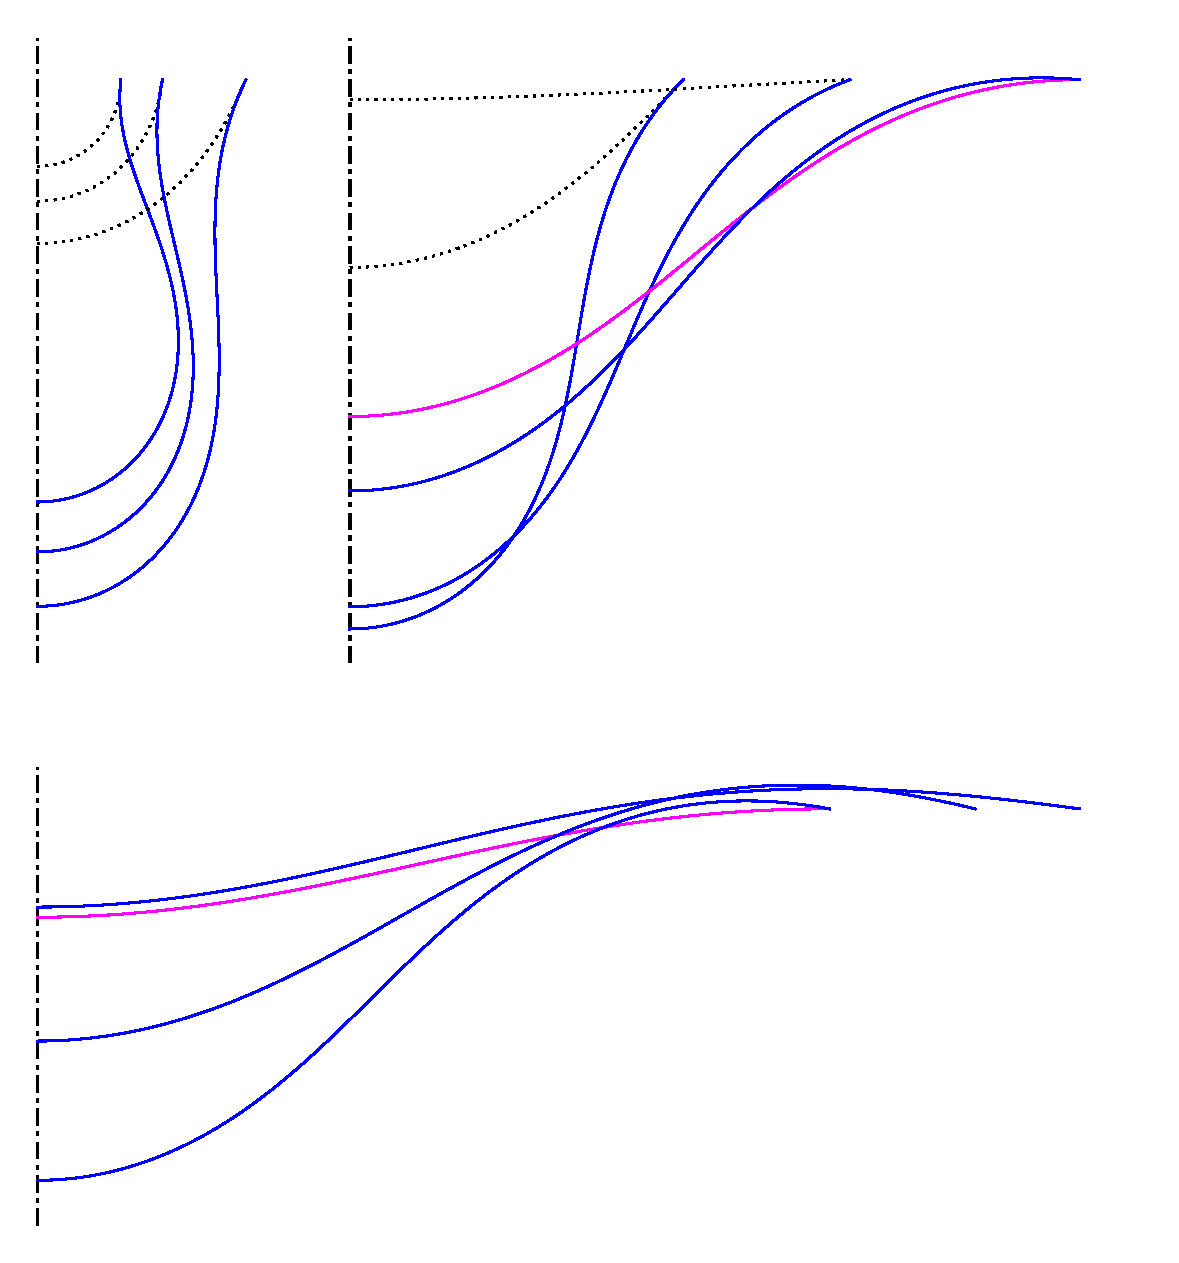
\includegraphics[width=0.6\linewidth]{Pending_Shapes.eps} 
$$
\caption{Pending drops : sample equilibrium shapes for 
$(a)$ $Bo =  0.4, 0.6, 1,$ ; 
$(b)$ $Bo = 1.6, 2.4, 3.6$ ;
$(c)$ $Bo = 3.8, 4.5, 5$. 
The profiles correspond to : maximum pressure (dotted) ; non-axisymmetric instability (grey ; magenta online) ; maximum volume (black ; blue online).
}
\end{figure}

\begin{figure}
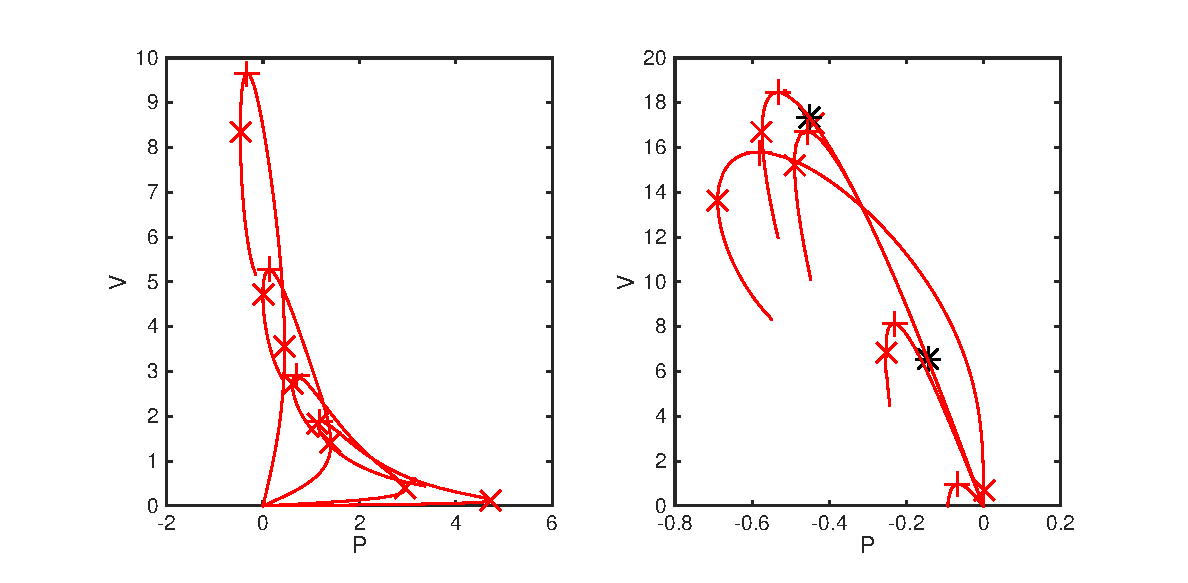
\includegraphics[width=\linewidth]{Pending_PV.eps} 
\caption{Pending drops : V-P curves for  
$(a)$ $Bo = 0.4, 0.6, 1, 1.6$ ; 
$(b)$ $Bo = 2.4, 3.6; 3.8, 4.5, 5$. 
The symbols correspond to : maximum (or minimum) pressure (x) ; non-axisymmetric instability (*) ; maximum volume (+).
}
\end{figure}


\begin{figure}
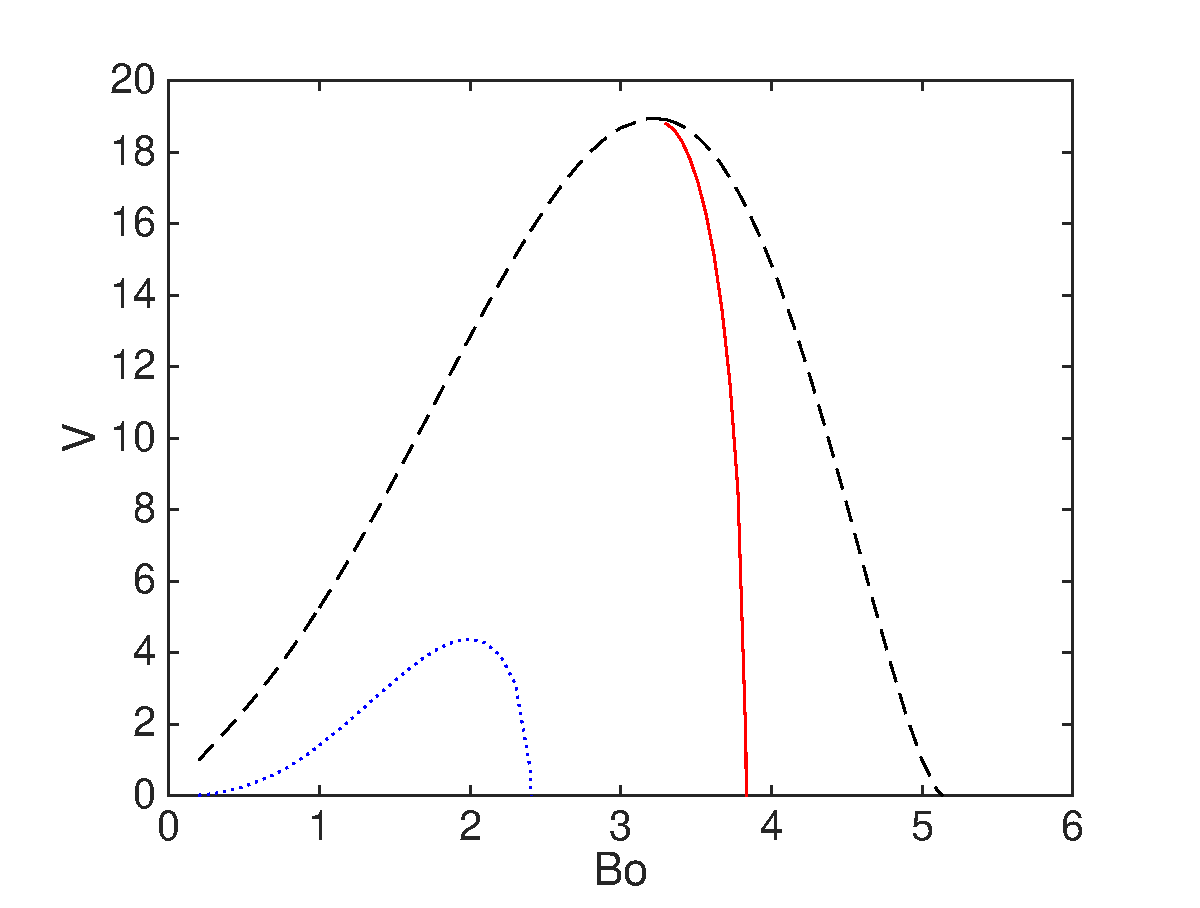
\includegraphics[width=.48\linewidth]{Pending_BoV.eps}
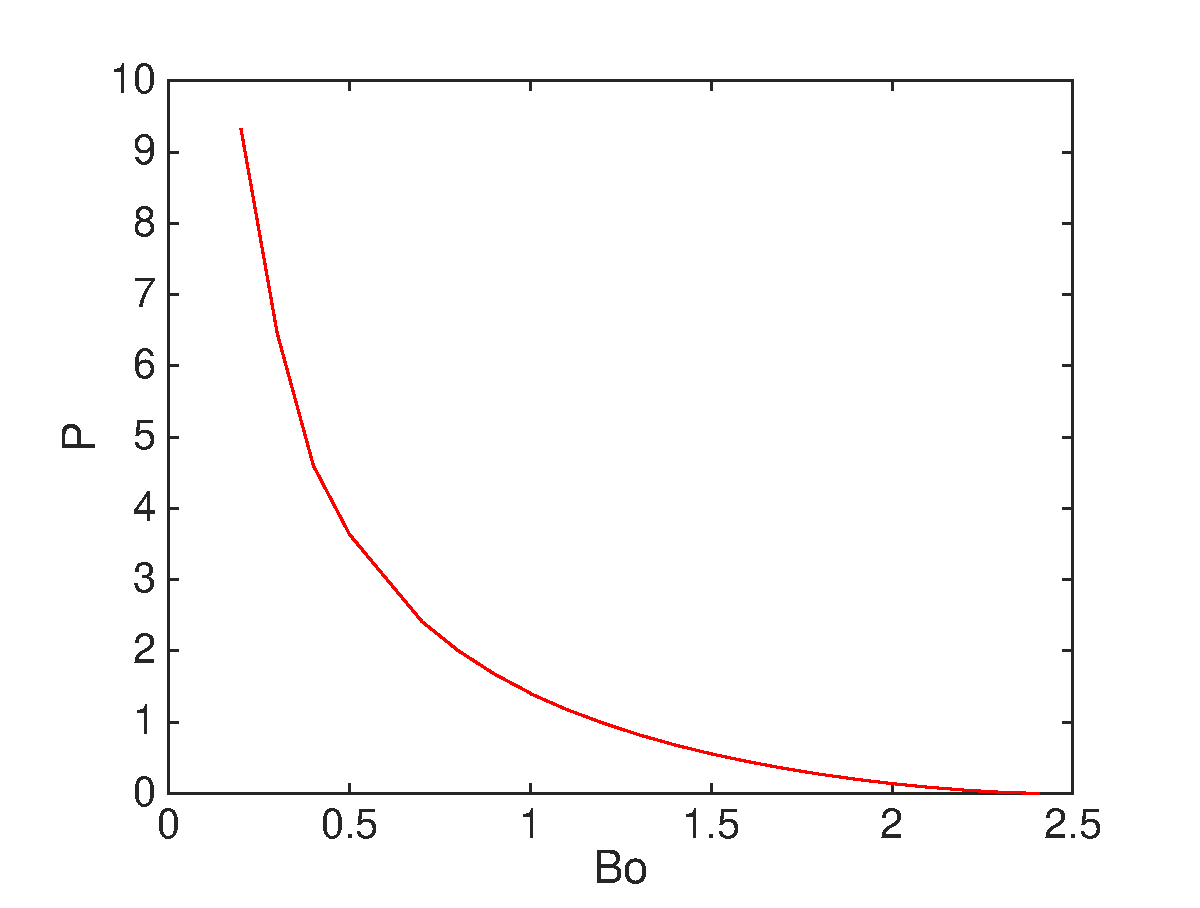
\includegraphics[width=.48\linewidth]{Pending_BoP.eps} 
\caption{
Pending drops : $(a)$ Volume $V$ corresponding to maximum volume (dashed line), 
non-axisymetric stability threshold (plain line), and maximum pressure (dotted line).
$(b)$ Maximum pressure $P$.
}
\end{figure}



\section{Spilling drops}


\begin{figure}
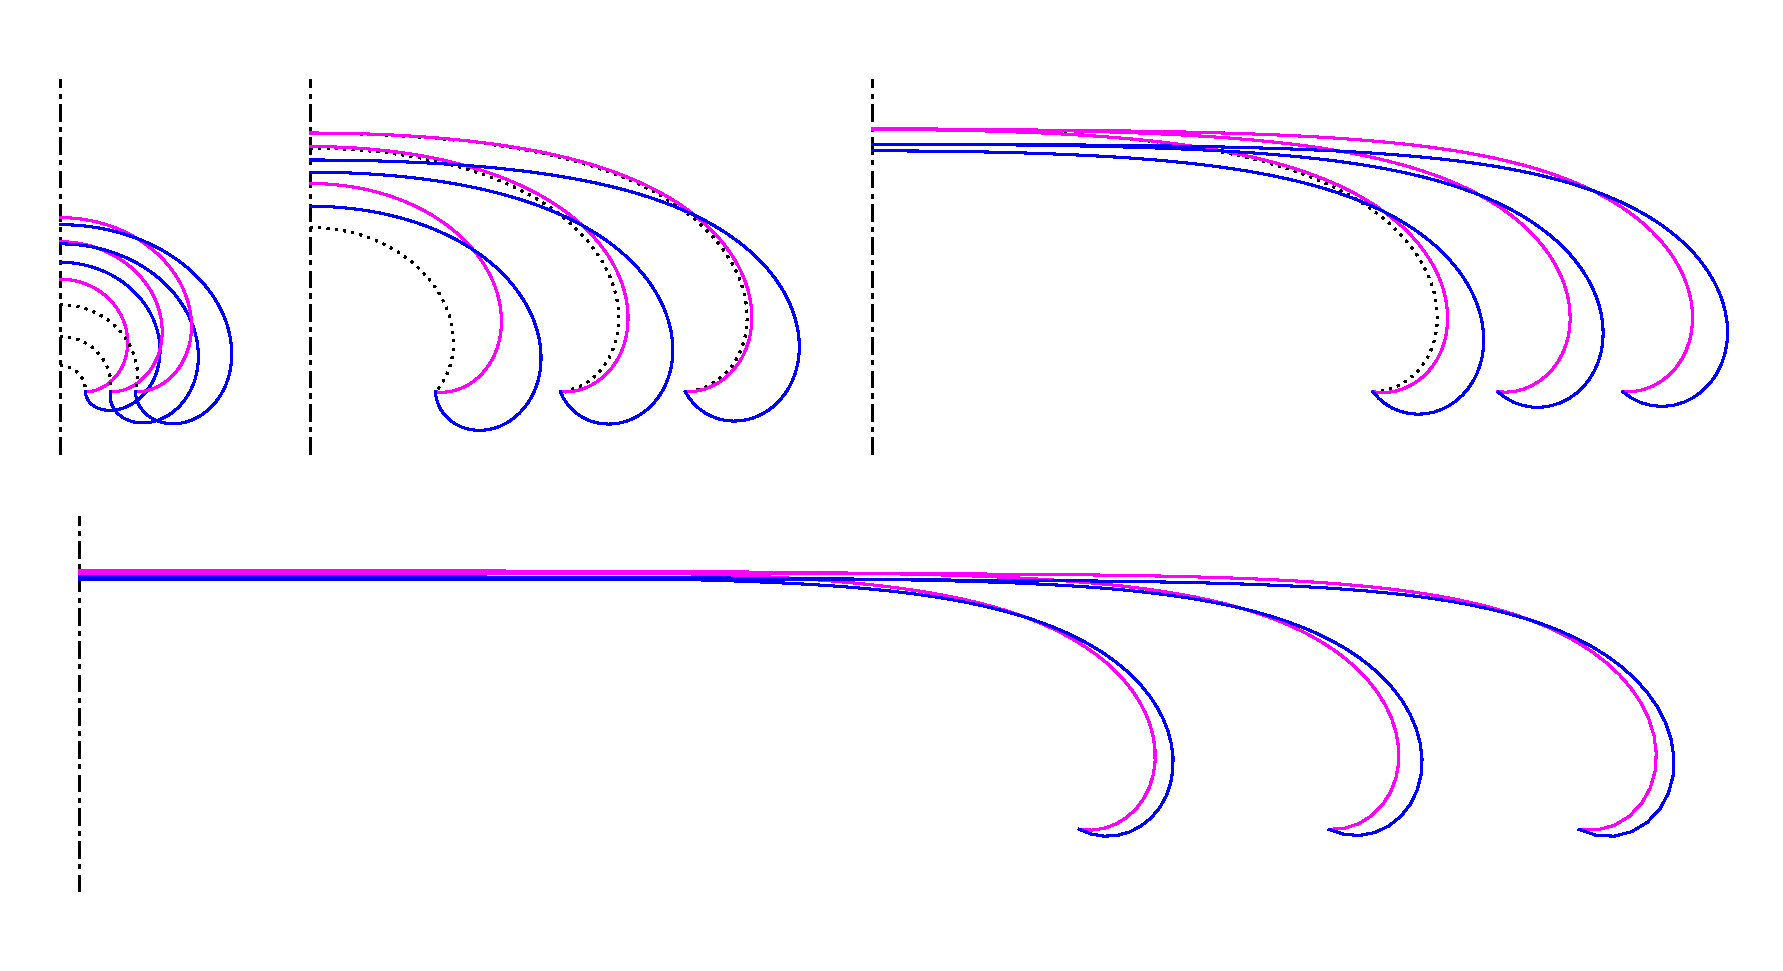
\includegraphics[width=\linewidth]{Sessile_Shapes.eps} 
\caption{Spilling drops : sample equilibrium shapes for 
$(a)$ $Bo = 0.2, 0.4, 0.6$ ; 
$(b)$ $Bo = 1, 2, 3$ ;
$(c)$ $Bo = 4, 5, 6$ ;
$(d)$ $Bo = 8, 10, 12$. 
In each case the three profiles correspond to : maximum pressure (magenta) ; non-axisymmetric instability (green) ; maximum volume (blue).
}
\end{figure}

\begin{figure}
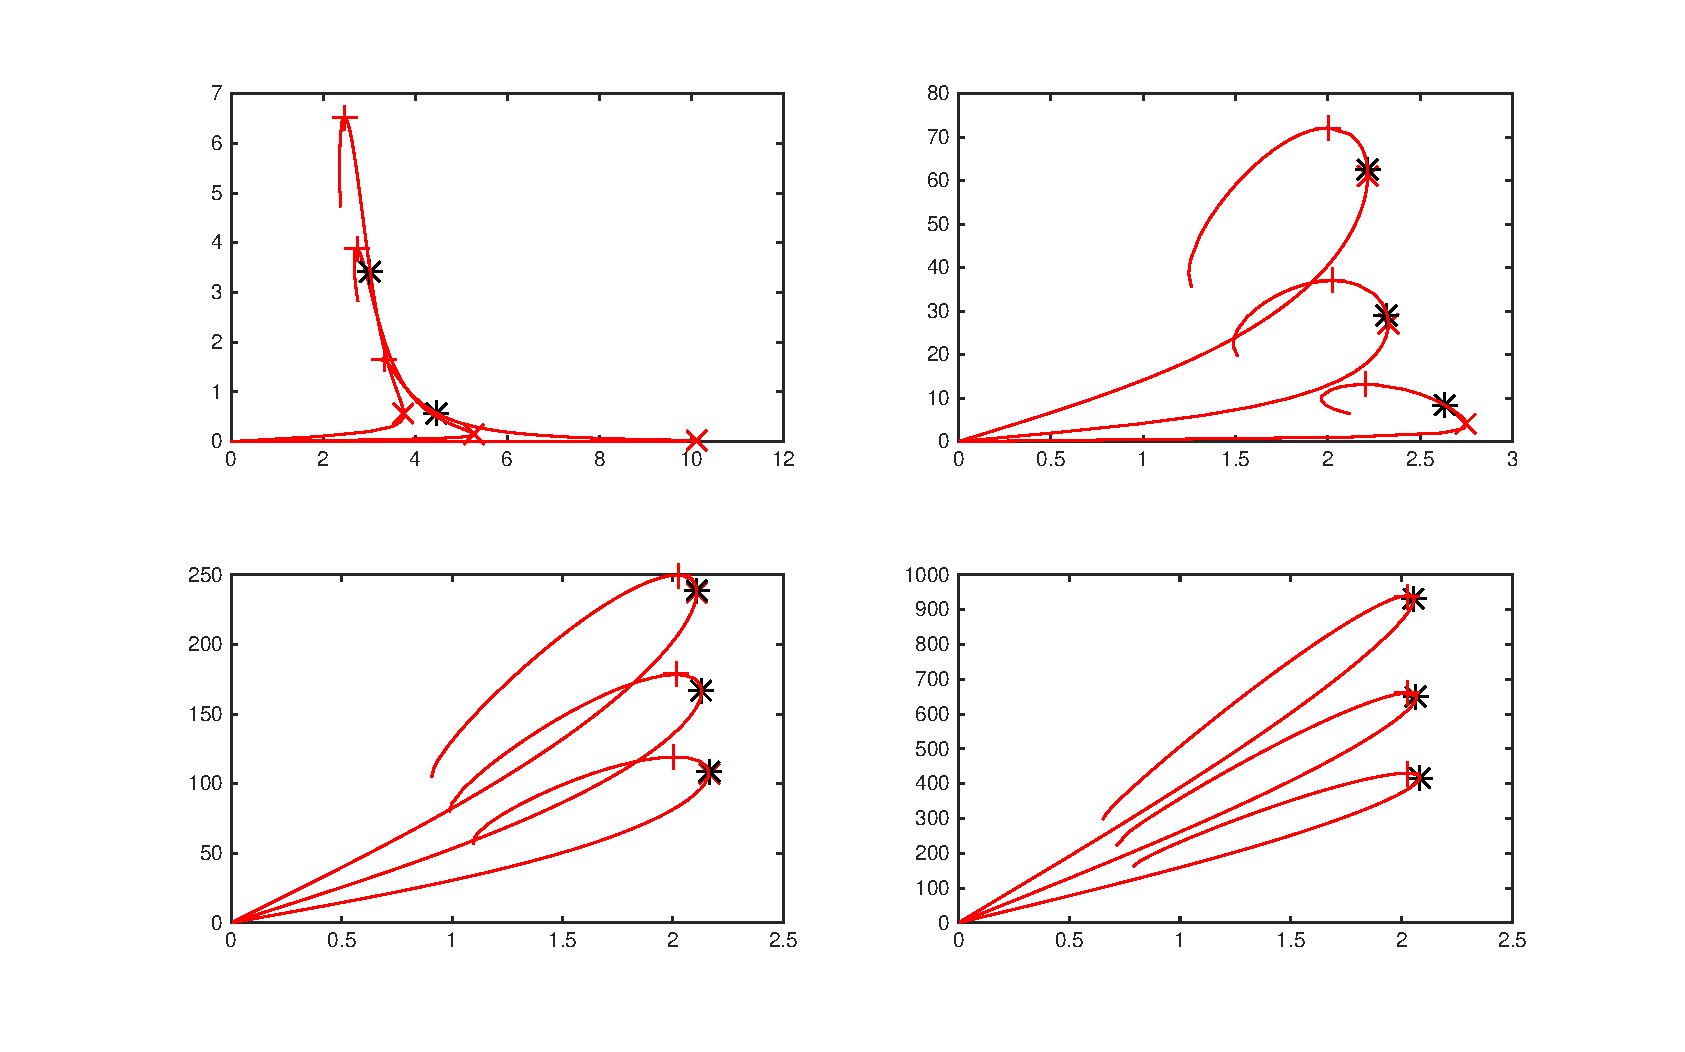
\includegraphics[width=\linewidth]{Sessile_PV.eps} 
\caption{Spilling drops : V-P curves for  
$(a)$ $Bo = 0.2, 0.4, 0.6$ ; 
$(b)$ $Bo = 1, 2, 3$ ;
$(c)$ $Bo = 4, 5, 6$ ;
$(d)$ $Bo = 8, 10, 12$. 
The symbols correspond to : maximum pressure (x) ; non-axisymmetric instability (*) ; maximum volume (+).
}
\end{figure}


\begin{figure}
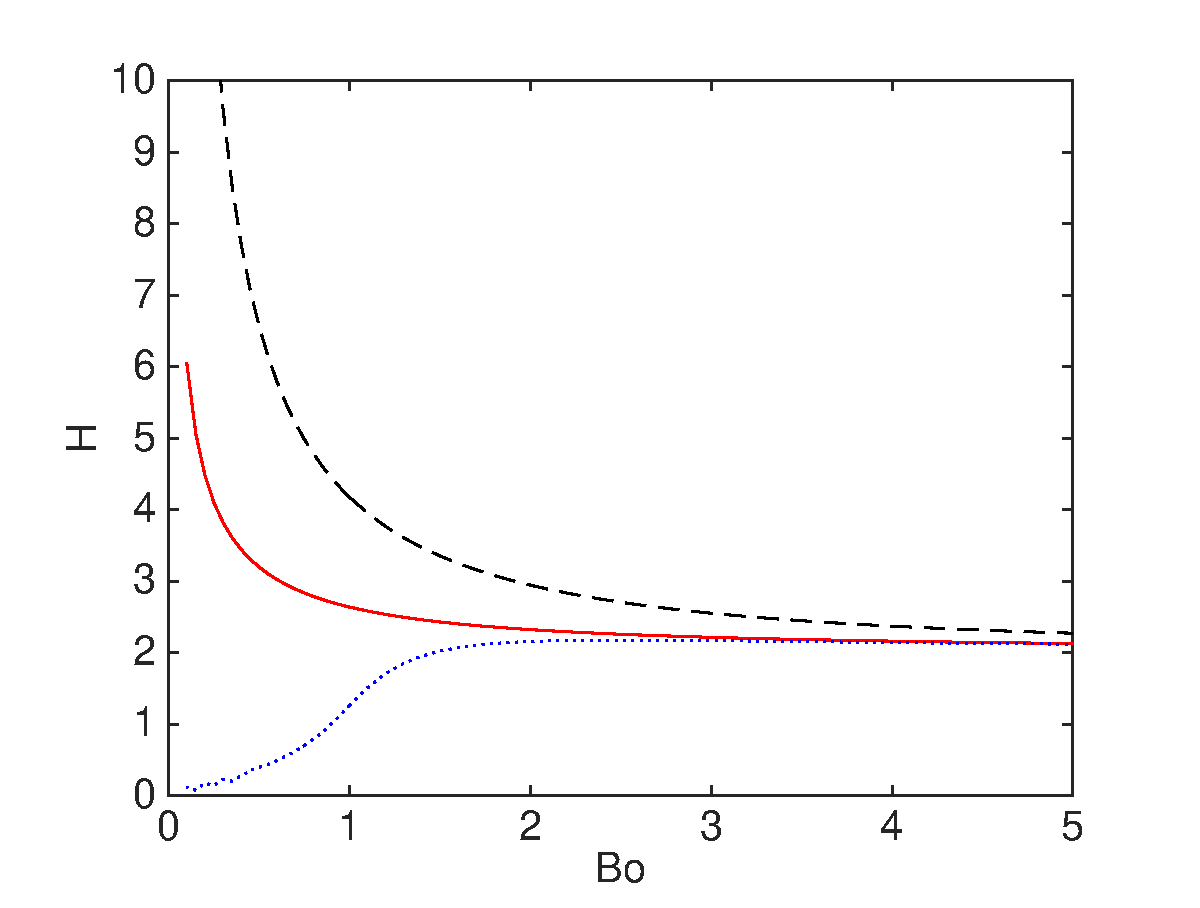
\includegraphics[width=.48\linewidth]{Sessile_BoV.eps}
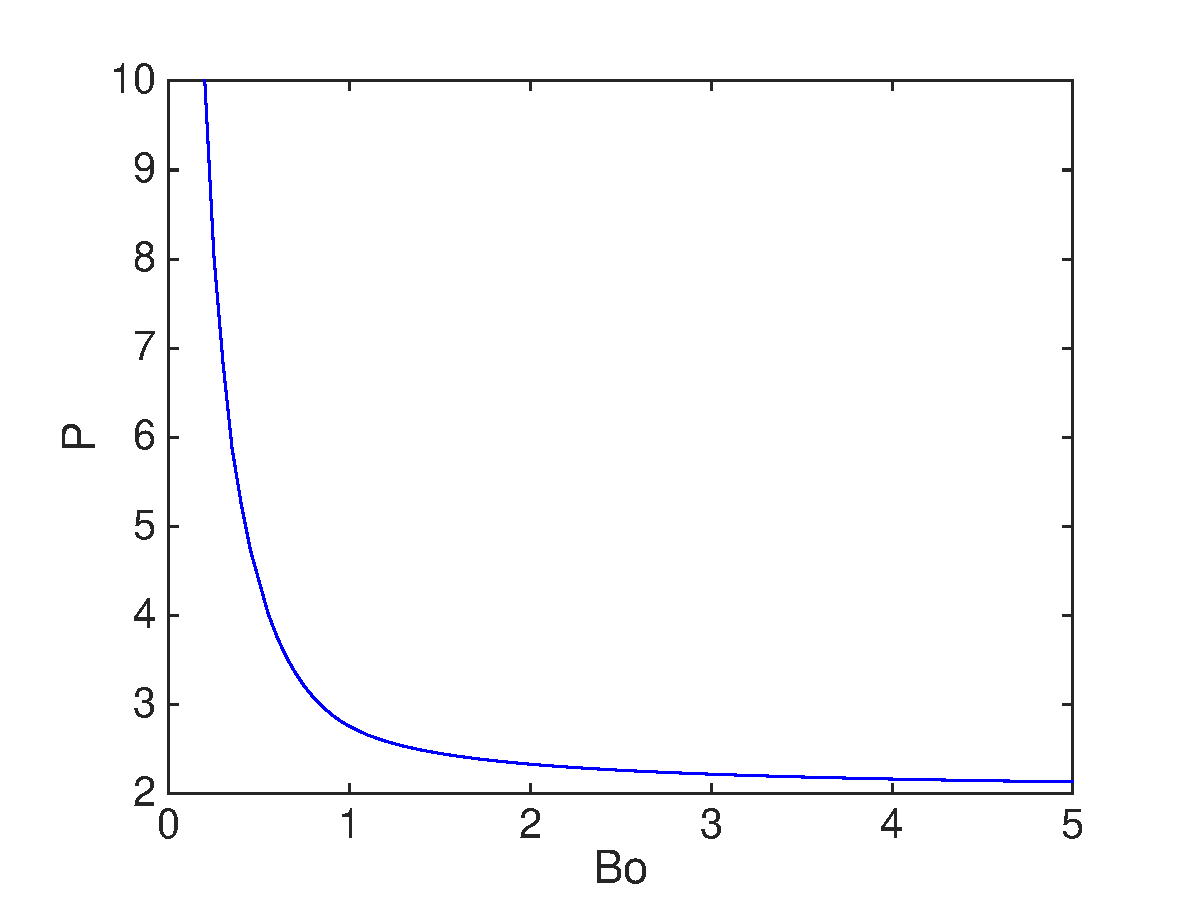
\includegraphics[width=.48\linewidth]{Sessile_BoP.eps} 
\caption{
Spilling drops : $(a)$ Equivalent height $H = V/(\pi Bo^2)$ corresponding to non-axisymetric stability threshold (plain line), maximum volume (dashed line), and maximum pressure (dotted line).
$(b)$ Maximum pressure $P$.
}
\end{figure}



\section{Liquid bridges (no gravity)}

\subsection{Equilibrium shapes}

The equilibrium shapes are computed through an iterative method, described in the appendix (see also Tong Lei Zhang's master). The program is implemented in Matlab language.
The continuation is done with taking as a control parameter either the pressure (=the curvature) inside the bridge (program \verb| Newton_P.m | ), or the volume (program \verb| Newton_V.m |).
The effect of gravity is also implemented.


Once the ratio $L/a$is fixed, the equilibrium shapes form a family which can be parametrized by either the pressure (or curvature), or the volume.

Figure 1 shows the Pressure/Volume relation for three cases ($L/a = 1.3 ; 2 ; 6$),
and figure 2 shows a few shapes in the $R-Z$ plane. Note that starting from the cylindrical bridge, the trend is different for short and long bridges : for short ones increasing the pressure (curvature) leads to an increase of the volume, while for long ones  increasing the pressure (curvature) leads to an decrease of the volume. In all cases, the curve passes through a state of minimum volume, and terminates at a green point where the shape asymptotes to two touching spheres.
We also identify in green the shape which has the same volume as this limit shape. In a coalescence process starting from two touching states, this is the final state, since the volume is conserved during the process and the initial state is unstable.

Note that this final state corresponds corresponds to larger volume than the cylindrical solution for long bridges, and to a smaller volume for short bridges.

The characteristics of these final states are respectively :
For $L/a=1.3$ : $[P,V] = [ -0.01257;  2.3296]$ ; 
For $L/a= 2$ : $[P,V] = [ 0.7428 ;  4.1888 ]$ ; 
For $L/a = 4$ : $[P,V] = [  0.9699 ; 14.6607]$ ;
For $L/a= 6$ : $[P,V] = [0.7926 ; 37.7]$.

Note also that in the case $L/a = 1.3$, the problem admits two solutions with zero pressure (or curvature), which correspond to classical catenoidal shapes. These cases are identified in blue.
 




\begin{figure}
\begin{tabular}{cc}
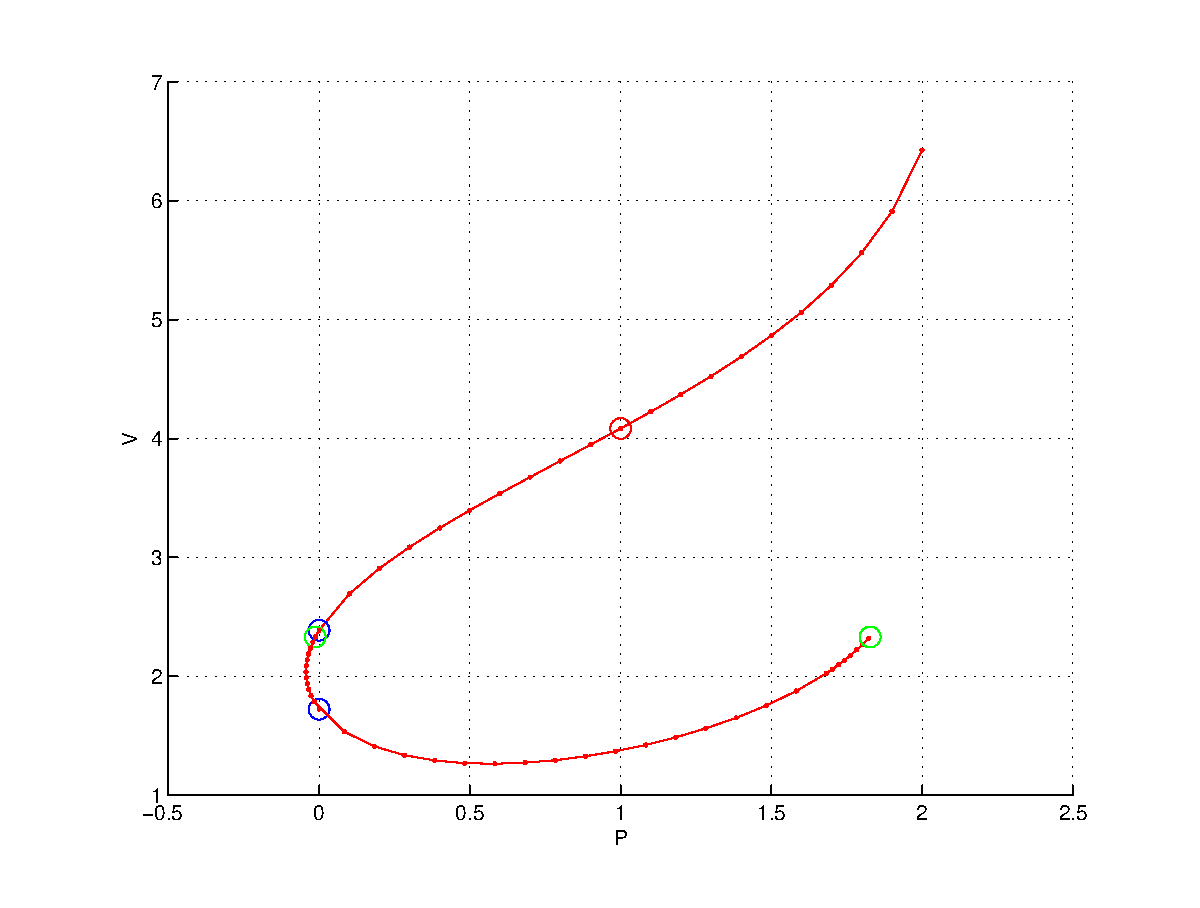
\includegraphics[width=.45\linewidth]{VPBridges_L1_3.eps} &
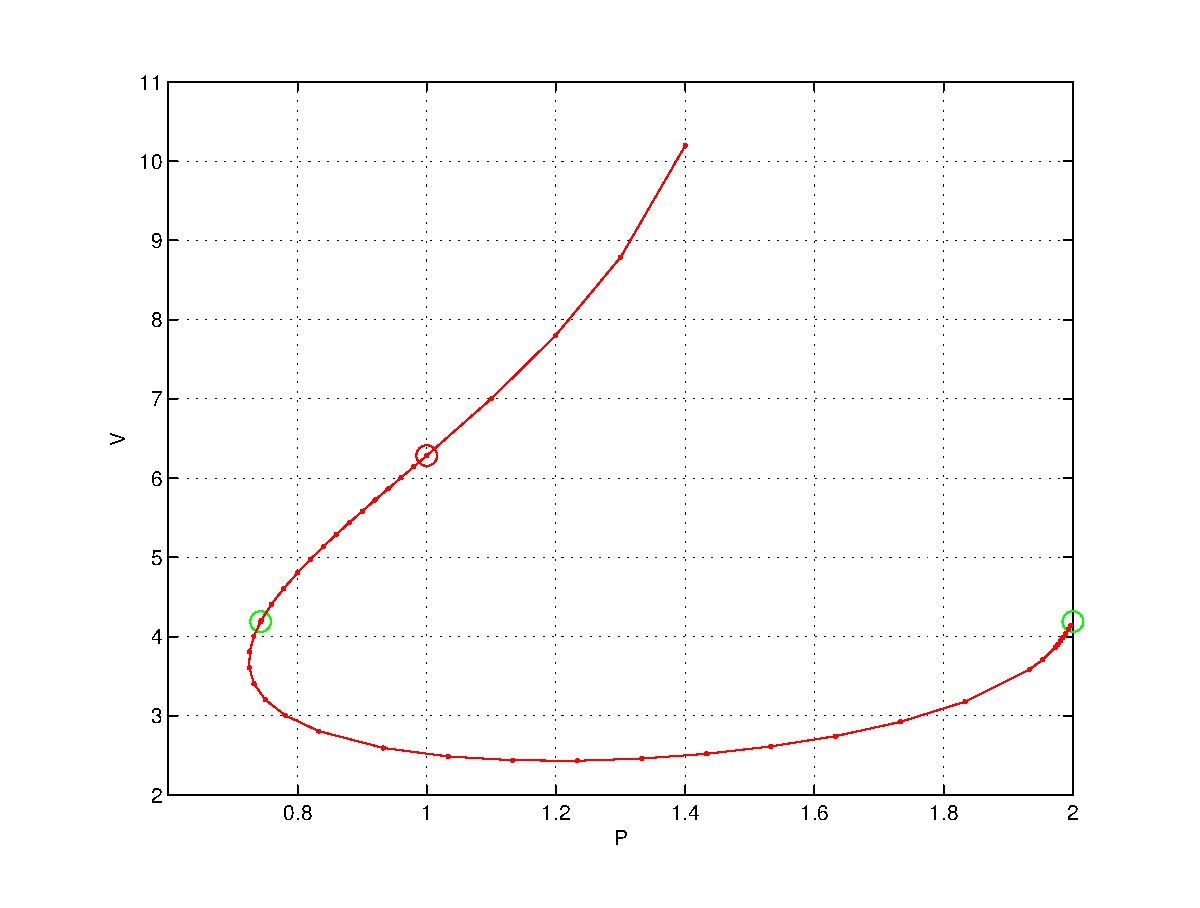
\includegraphics[width=.45\linewidth]{VPBridges_L2.eps} \\
$(a)$ : $L/a = 1.3$ & $(b)$ : $L/a = 2$ \\
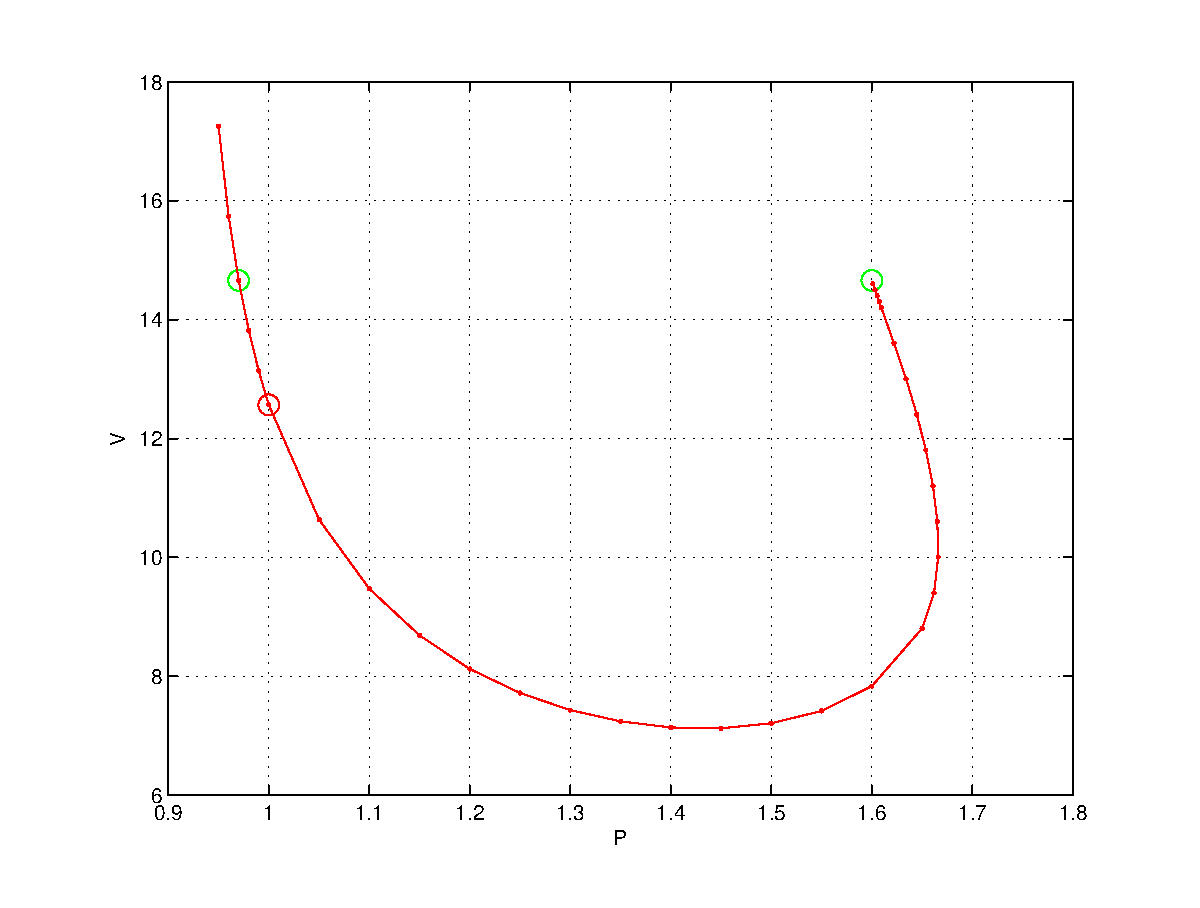
\includegraphics[width=.45\linewidth]{VPBridges_L4.eps} & 
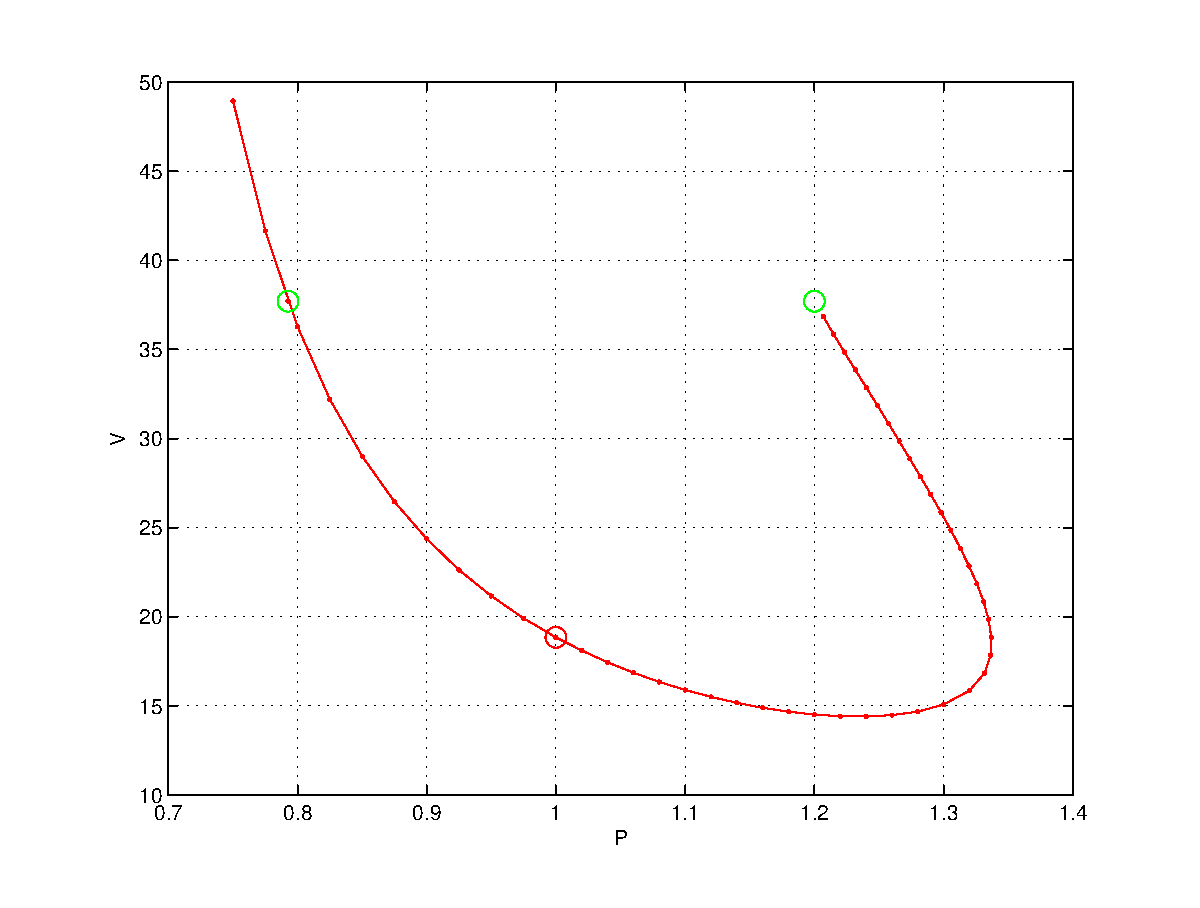
\includegraphics[width=.45\linewidth]{VPBridges_L6.eps} \\
$(c)$ : $L/a = 4$ & $(d)$ : $L/a = 6$ \\
\end{tabular}
\caption{Pressure-volume relations for equilibrium shapes, for $L/a= 1.3; 2; 4$ and $6$. Circles identify the cylindrical shape (red), the limit shape of touching spheres (green), the shape with same volume (green), and (for $L/a= 1.3$) the catenoidal shapes (blue). }
\end{figure}

\begin{figure}
$$
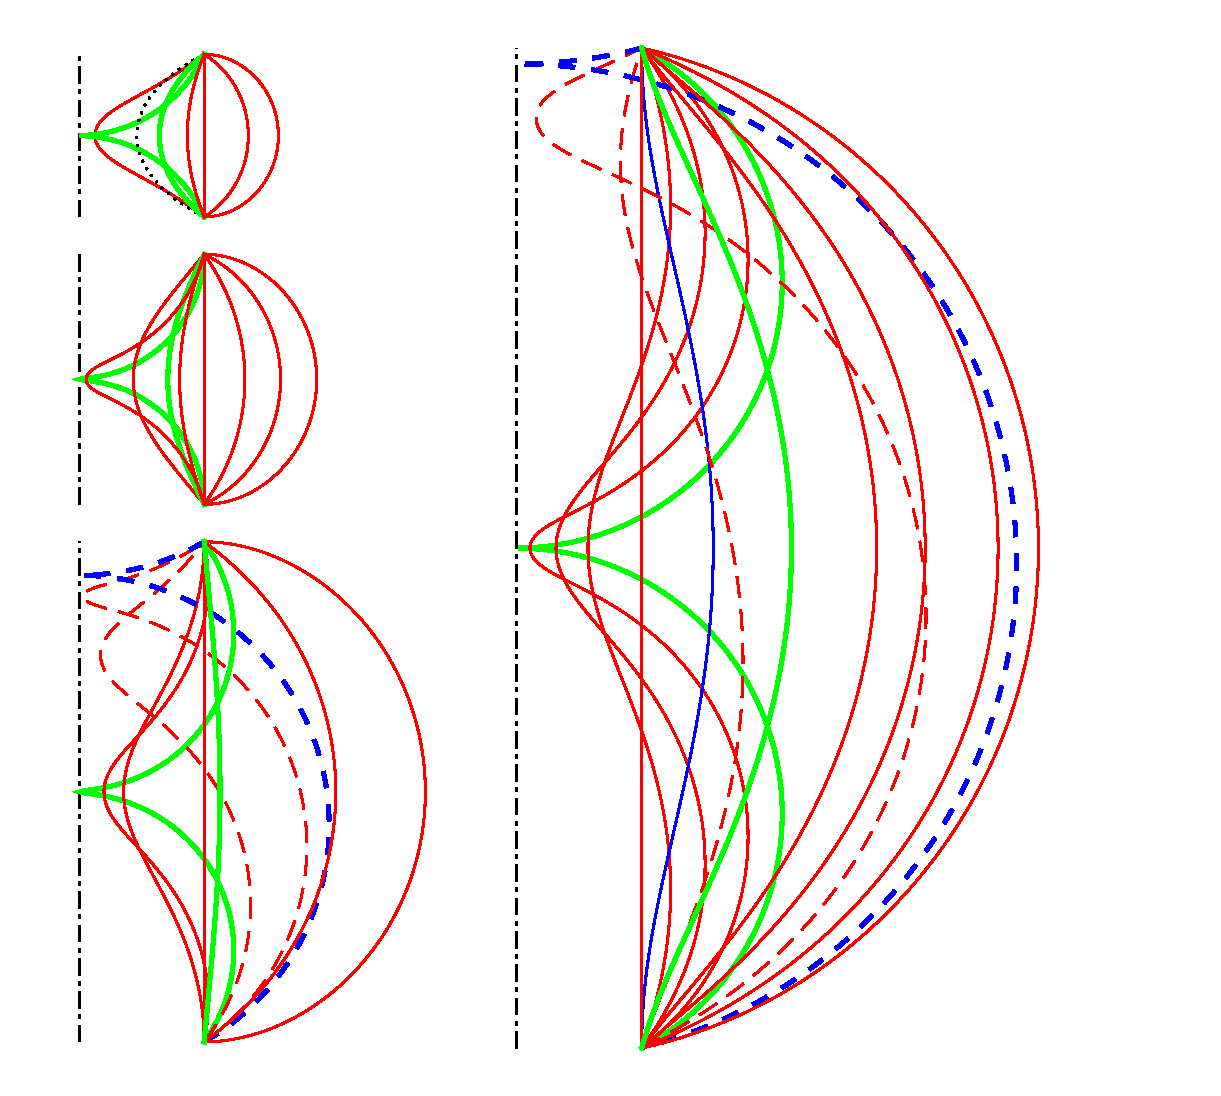
\includegraphics[width=.8\linewidth]{Bridges_Shapes.eps}
$$
\caption{Sample equilibrium shapes of liquid bridges with zero gravity, 
for $(a)$ $L/a= 1.3$, $(b)$ $L/a=2$, $(c)$ $L/a=4$, and $(d)$ $L/a=8$.
In all cases, the thick, grey (green online) contours correspond to the limit case of two touching spheres of equal size and to the shape with same volume ; in $(a)$ the dotted line corresponds to  a catenoid shape;
in $(c)$ and $(d)$ the dashed contours are asymmetric shapes and the thick, dashed one is the limit case of two touching spheres of unequal size. }
\end{figure}



\subsection{Frequency calculations}

\begin{table}
\begin{center}
\begin{tabular}{ll|ll|ll|}
$L/a$ & shape & $(0,A)$ & $(0,S)$ & $(1,S)$ & $(1,A)$ \\
\hline
2 & cyl. 		& 3.26637 &  7.53435  &   1.49269 &  4.7160\\
2 & noncyl		&  2.37693 &  6.25495 & 1.40023 &  4.22306 \\
\hline
4 & cyl. 		& 7.346183e-01  & 2.132444e+00  & 4.996549e-01  & 1.496437e+00\\
4 & noncyl		& 7.933437e-01  & 2.215907e+00  & 4.697427e-01  & 1.490868e+00\\
\hline
6 & cyl. 		& 1.298953e-01 & 8.451902e-01	&   2.907411e-01   &  7.828465e-01\\
6 & noncyl		& 3.579927e-01 & 1.107705e+00 	&  2.218312e-01  &  7.857503e-01 \\
\hline
\end{tabular}
\end{center}
\caption{Some values of Eigenfrequencies ($m=1$ to be checked)}
\end{table}


 The table gives a few values of the frequencies with cylindrical and non-spherical shape
 (corresponding to green point in figure 1).
 
 We can see that the departure from the cylindrical shape leads to an increase of frequencies for long bridges and to a decrease for short bridges, mostly for axisymetric modes. The effect is less pronounced on non-axisymetric modes.
  
 



Eigenfrequencies for $m=0$ modes are given in figure 3 as function of  pressure, for $L/a=4$.

\begin{figure}
$$
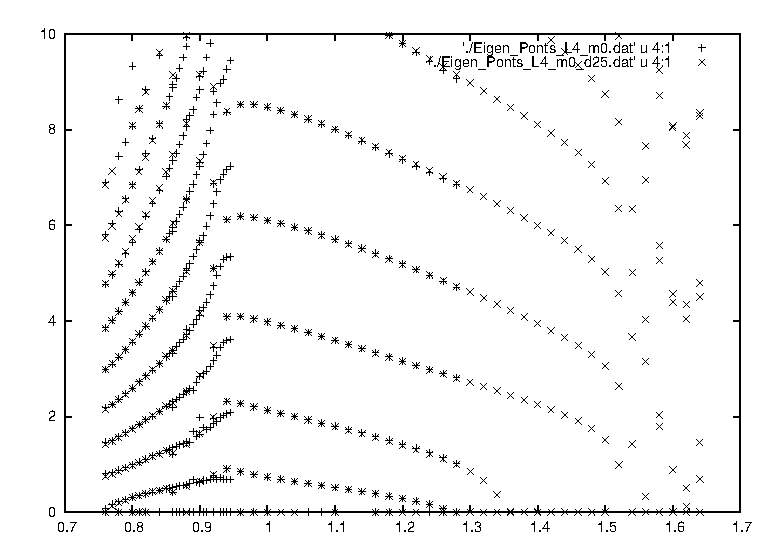
\includegraphics[width=.5\linewidth]{Eigenvals_TestL4.eps}
$$
\caption{Frequencies of axisymmetric modes ($L/a=4$) : ANCIENNE VERSION.
Petit problème a régler aux alentour de $P=0.94$ => ça a l'air réglé avec  nouvelle version avec densité suffisante (45)}
\end{figure}


TO BE CONTINUED....

     
            
            
            
            
            
            
            
            
            
%\begin{abstract}
%\end{abstract}
%\begin{keywords}
%\end{keywords}


\clearpage

\appendix


\section{Stability and oscillation frequencies of cylindrical liquid bridges}

\subsection{Problem formulation}

We consider a  cylindrical liquid bridge of radius $a$ and length $L$. 

For nondimensionalisation we set $a=1,\rho=1,\gamma=1$.

The unknown are a potential $\phi$ defined in the volume, and a normal displacement $\eta$ defined on the surface (extending for $x=-L/2$ to $x = +L/2$):

$$ {\bf u} = \epsilon \nabla \phi(x,r) e^{i (m \theta + \omega t)}$$
$$ r = a + \epsilon \eta(x)  e^{i (m \theta + \omega t)}$$


Equations :

\bea
\Delta \phi &=& 0, \\
\partial_x \phi &=& 0 \quad \mbox{ for } x= 0 \mbox{ and } x=L, \\
\partial_r \phi &=& i \omega \eta \quad \mbox{ for } r=a, \\
\gamma K_1 = \gamma (-\partial_x^2 + m^2/a^2   -1/a^2) \eta &=&  i \omega \phi \quad \mbox{ for } r=a, \\
\eta &=& 0  \quad \mbox{ for } x= 0 \mbox{ and } x=L. \\
\eea

\subsection{Analytical solution}

The method is in the line of that of Henderson \& Miles (1994) for sloshing modes  in a cylindrical container 
with fixed contact line.

We first expand the potential in the following form (which automatically satisfies the boundary conditions at $x = 0,L$) :

\bea
\phi &=& \sum\limits_{n=0}^{\infty} \phi_n \cos (  k_n x ) \frac{I_m(k_n r)}{I_m(k_n a)}
 \\
 &=& 
 \sum\limits_{n=0}^{\infty} \phi_{2n} {(-1)}^n \cos (  k_{2n} x' ) \frac{I_m(k_{2n} r)}{I_m(k_{2n} a)}
 + 
 \sum\limits_{n=0}^{\infty} \phi_{2n+1} {(-1)}^{n} \sin (  k_{2n+1} x' ) \frac{I_m(k_{2n+1} r)}{I_m(k_{2n+1} a)}
 \eea
 
where $k_n = n \pi /L$.

The second expression is in terms of $x' = x-L/2$ which spans the bridge from $-L/2$ to $L/2$. In terms of this centered variable, this expression allows to separate the symmetrical and anti symmetrical components, which contain respectively only even and odd terms.
However, for the remainder it is simpler to stay with the first expression in terms of $x$, in order to avoid mixing between sines and cosines.



We first work with the dynamic boundary condition which can be written in the following form :

\be
\gamma (-\partial_x^2 + m^2/a^2   -1/a^2) \eta =  \sum\limits_{n=0}^{\infty}(i \omega) \phi_n \cos (  k_n x )
\label{eq:etaD}
\ee

Unless if the right-hand side contains resonant terms (see below), the solution of this equation will be generally written as follows :


\be
\eta = \sum\limits_{n=0}^{\infty} A_{n}  \cos (  k_{n} x ) -  \left (A_s C_s(x) + A_a C_a(x) \right)
\label{eq:eta1}
\ee

We recognize two parts : the first is the solution proportional to the forcing terms, with amplitudes $A_n$
given as follows :

$$A_n = \frac{-i \omega \phi_n}{\gamma (k_n^2 a^2 +m^2 -1)} $$

The second part is the solution to the homogeneous equation. This part contains two auxiliary functions, noted $C_s(x)$ and $C_a(x)$. These functions are chosen so that $C_s(x)$ is symmetric and $C_a(x)$ is  
antisymmetric, and are normalized by $C_s(0) = C_a(0)= 1$. Physically, these two functions represent displacements of the free surface which do not modify the mean curvature.
The expressions for these functions depends upon $m$ and will be given below.


We now consider the kinematic boundary condition, which yields :
\be
\eta = (i \omega)^{-1} 
\sum\limits_{n=0}^{\infty} \phi_n \cos (  k_n x ) T_n, \quad 
\mbox{ with } T_n = \frac{I'_m(k_{n} a)}{I_m(k_{n} a)}
\ee
Using the previous expression for $A_n$, this expression leads to :


\be 
\eta = \sum\limits_{n=0}^{\infty} \left( \frac{\omega^*_{n}}{\omega}\right)^2 A_n \cos (  k_n x )
\label{eq:eta2}
\ee
where
$$
(\omega^*_{n})^2   = \frac{\gamma}{\rho a^3} \left( k_n^2 + m^2 - 1 \right) T_n
$$
are the "free" frequencies (eigenfrequencies that would be obtained if we relax the fixed-line condition).




We now have two different expressions for $\eta(x)$, namely (\ref{eq:eta1}) and (\ref{eq:eta2}), and must equate them. One clearly sees that if the complementary functions are absent, the solution is trivially
$\omega = \omega^*_{n}$ : the Fourier components are uncoupled and the frequencies are those of "free problem". These modes do not verify the condition of fixed line, but instead they verify $\partial_x \eta =0 $ ; physically this represents a bridge located between two parallel planes and allowed to slip along them.

When the fixed constraint is imposed, the complementary functions have to be introduced. To equate the two expressions for $\eta$, these functions have to be decomposed along the Fourier basis. The decomposition is as follows :


$$
C_s(x) = \sum\limits_{n=0}^{\infty} C^s_{n} \cos (  k_{2n} x ) 
$$

$$
C_a(x) = \sum\limits_{n=0}^{\infty} C^a_{n} \cos (  k_{2n+1} x )
$$

The Fourier coefficients will be given below.
We can now work separately for the symmetric and antisymmetric parts of the expression for $\eta$.
For symmetric perturbations, equating the Fourier coefficients leads to :

\be 
\left( \frac{\omega^*_{2n}}{\omega}\right)^2 A_{2n} = A_{2n} + A_s C^s_n %\mbox{ for } n\ge 0.
\label{eq:AnAs}
\ee
Which can also be written :


$$
A_{2n}  = A_c C^s_{n} \left( \frac{\omega^2}{\omega^2- \omega^*_{2n}} \right) 
$$

It remains to sum over all indices $n$, and recognize that $\sum A_{2n} = A_s$
(which comes from the fixed-line condition $\eta(0) = 0$), to get the following dispersion relation :



\be
F_s(\omega^2)=  \sum C^s_{n} \left( \frac{\omega^2}{\omega^2- \omega^*_{2n}} \right)  = 1
\label{eq:RDs}
\ee

The case of antisymmetric modes is similar and yields 

\be
F_a(\omega^2) = \sum C^a_{n} \left( \frac{\omega^2}{\omega^2- \omega^*_{2n+1}} \right)  = 1.
\label{eq:RDa}
\ee


We can note that the functions $F_s$ and $F_a$ change sign through a infinite branch at the "free frequencies" $\omega^*_{n}$ and are monotonous between these roots  (check ?) ; so we can conclude that the frequencies for the fixed-line problem lie between those for the free-line problem.




\subsection{Details}

\begin{itemize}

\item
For $m=0$ , the auxiliary functions are given as 

\be
C_s(x) = \frac{\cos(x-L/2)}{\cos(L/2)} ; \quad C_a(x) = \frac{\sin(L/2-x)}{\sin(L/2)}
\ee

The fourrier coefficients for these functions are as follows :

$$
C^s_{n} = \frac{4 L}{L^2 - \pi^2 (2n)^2} \tan (L/2) \quad \mbox{ if } n\ne 0
$$
$$
C^s_0 = \frac{2}{L} \tan (L/2)
$$
$$
C^a_{n} = - \frac{4 L}{L^2 - \pi^2 (2n+1)^2} \cot (L/2) 
$$

Note that if $L = n \pi$, the problem for $\eta$ becomes non-homogenous  and a special treatment is required. However these case are of no particular significance, so we omit the details.


\item
For $m\ge 2$ , the auxiliary functions are given as 


\be
C_s(x) = \frac{\cosh(\mu (x-L/2))}{\cosh(\mu L/2)} ; \quad C_a(x) = \frac{\sinh(\mu (L/2-x))}{\sinh(\mu L/2)}
\ee

The fourrier coefficients for these functions are as follows :

$$
C^s_{n} = \frac{4 L\mu }{\mu^2 L^2 + \pi^2 (2n)^2} \tanh (\mu L/2) \quad \mbox{ if } n\ne 0
$$
$$
C^s_0 = \frac{2}{L} \tanh (L/2)
$$
$$
C^a_{n} = \frac{4 L\mu }{\mu^2 L^2 + \pi^2 (2n+1)^2} \coth (\mu L/2)
$$

\item The case $m=1$ requires a specific treatment. In that case, the left-hand side of the equation (\ref{eq:etaD}) is simply $\partial_x^2 \eta = 0$, whose homogenous solutions are constants and linear functions, but the right-hand side contains the constant term $i \omega \phi_0$ which proportional to the homogenous solution, hence resonant. In that case,
the auxiliary function $C^s(x)$ has to be taken as the response to this resonant term, namely 
$$
C_s(x) = (2x/L-1)^2
$$
The antisymmetric auxiliary function is $C_a(x)$ and is not resonant, and is taken as :
$$
C_a(x) = (1- 2x/L)
$$

The Fourier coefficients for these auxiliary functions are :
$$
C^s_{n} = \frac{16}{\pi^2 n^2} 
\quad \mbox{ if } n\ne 0
$$
$$
C^s_0 = 1/3
$$
$$
C^a_{n} = \frac{8}{\pi^2 n^2} 
$$        
        

The solution to the antisymmetric problem is still given by \ref{eq:RDa}.

 
The symmetric problem is slightly different. 
In this case, the expressions for $A_n$ given above (\ref{eq:AnAs}) are still valid for $n\ne 0$, but the case $n=0$ is different, and the expressions has to be replaced by :
$$
A_0 = 
\left( \frac{8}{\pi^2L^2} + C_0^s \right) A_s 
$$

Hence in this case the dispersion relation reads :

\be
F_s(\omega^2)= 
\left( \frac{8}{\pi^2L^2} + \frac{1}{3} \right) + 
\sum\limits_{n=1}^{\infty} C^s_{n} \left( \frac{\omega^2}{\omega^2- \omega^*_{2n}} \right)  = 1
\label{eq:RDsm1}
\ee

\end{itemize}

%\end{document} 
 

\section{Calcul de la courbure}

VERIFIER LES SIGNES

\subsection{Formules de base}

\begin{figure}
% This is file JFM2esam.tex
% first release v1.0, 20th October 1996
%       release v1.01, 29th October 1996
%       release v1.1, 25th June 1997
%       release v2.0, 27th July 2004
%   (based on JFMsampl.tex v1.3 for LaTeX2.09)
% Copyright (C) 1996, 1997 Cambridge University Press

\NeedsTeXFormat{LaTeX2e}

\documentclass{jfm}
\usepackage[T1]{fontenc}
%\documentclass[referee]{jfm} %for double spaced output for submission

% See if the author has AMS Euler fonts installed: If they have, attempt
% to use the 'upmath' package to provide upright math.

\usepackage{graphicx}
\usepackage{natbib}
\usepackage{rotate}
\usepackage{epstopdf}
\usepackage{pstricks}

\ifCUPmtlplainloaded \else
  \checkfont{eurm10}
  \iffontfound
    \IfFileExists{upmath.sty}
      {\typeout{^^JFound AMS Euler Roman fonts on the system,
                   using the 'upmath' package.^^J}%
       \usepackage{upmath}}
      {\typeout{^^JFound AMS Euler Roman fonts on the system, but you
                   dont seem to have the}%
       \typeout{'upmath' package installed. JFM.cls can take advantage
                 of these fonts,^^Jif you use 'upmath' package.^^J}%
       \providecommand\upi{\pi}%
      }
  \else
    \providecommand\upi{\pi}%
  \fi
\fi

% See if the author has AMS symbol fonts installed: If they have, attempt
% to use the 'amssymb' package to provide the AMS symbol characters.

\ifCUPmtlplainloaded \else
  \checkfont{msam10}
  \iffontfound
    \IfFileExists{amssymb.sty}
      {\typeout{^^JFound AMS Symbol fonts on the system, using the
                'amssymb' package.^^J}%
       \usepackage{amssymb}%
       \let\le=\leqslant  \let\leq=\leqslant
       \let\ge=\geqslant  \let\geq=\geqslant
      }{}
  \fi
\fi

% See if the author has the AMS 'amsbsy' package installed: If they have,
% use it to provide better bold math support (with \boldsymbol).

\ifCUPmtlplainloaded \else
  \IfFileExists{amsbsy.sty}
    {\typeout{^^JFound the 'amsbsy' package on the system, using it.^^J}%
     \usepackage{amsbsy}}
    {\providecommand\boldsymbol[1]{\mbox{\boldmath $##1$}}}
\fi


%%% Example macros (some are not used in this sample file) %%%

% For units of measure
\newcommand\dynpercm{\nobreak\mbox{$\;$dyn\,cm$^{-1}$}}
\newcommand\cmpermin{\nobreak\mbox{$\;$cm\,min$^{-1}$}}


% Various bold symbols
\providecommand\bnabla{\boldsymbol{\nabla}}
\providecommand\bcdot{\boldsymbol{\cdot}}
\newcommand\biS{\boldsymbol{S}}
\newcommand\etb{\boldsymbol{\eta}}

% For multiletter symbols
\newcommand\Real{\mbox{Re}} % cf plain TeX's \Re and Reynolds number
\newcommand\Imag{\mbox{Im}} % cf plain TeX's \Im
\newcommand\Rey{\mbox{\textit{Re}}}  % Reyno\usepackage{graphicx}lds number
\newcommand\Pran{\mbox{\textit{Pr}}} % Prandtl number, cf TeX's \Pr product
\newcommand\Pen{\mbox{\textit{Pe}}}  % Peclet number

% For sans serif characters:
% The following macros are setup in JFM.cls for sans-serif fonts in text
% and math.  If you use these macros in your article, the required fonts
% will be substitued when you article is typeset by the typesetter.
%
% \textsfi, \mathsfi   : sans-serif slanted
% \textsfb, \mathsfb   : sans-serif bold
% \textsfbi, \mathsfbi : sans-serif bold slanted (doesnt exist in CM fonts)
%
% For san-serif roman use \textsf and \mathsf as normal.
%
\newcommand\ssC{\mathsf{C}}    % for sans serif C
\newcommand\sfsP{\mathsfi{P}}  % for sans serif sloping P
\newcommand\slsQ{\mathsfbi{Q}} % for sans serif bold-sloping Q

% Hat position
\newcommand\hatp{\skew3\hat{p}}      % p with hat
\newcommand\hatR{\skew3\hat{R}}      % R with hat
\newcommand\hatRR{\skew3\hat{\hatR}} % R with 2 hats
\newcommand\doubletildesigma{\skew2\tilde{\skew2\tilde{\Sigma}}}
%       italic Sigma with double tilde

% array strut to make delimiters come out right size both ends
\newsavebox{\astrutbox}
\sbox{\astrutbox}{\rule[-5pt]{0pt}{20pt}}
\newcommand{\astrut}{\usebox{\astrutbox}}

\newcommand\GaPQ{\ensuremath{G_a(P,Q)}}
\newcommand\GsPQ{\ensuremath{G_s(P,Q)}}
\newcommand\p{\ensuremath{\partial}}
\newcommand\tti{\ensuremath{\rightarrow\infty}}
\newcommand\kgd{\ensuremath{k\gamma d}}
\newcommand\shalf{\ensuremath{{\scriptstyle\frac{1}{2}}}}
\newcommand\sh{\ensuremath{^{\shalf}}}
\newcommand\smh{\ensuremath{^{-\shalf}}}
\newcommand\squart{\ensuremath{{\textstyle\frac{1}{4}}}}
\newcommand\thalf{\ensuremath{{\textstyle\frac{1}{2}}}}
\newcommand\Gat{\ensuremath{\widetilde{G_a}}}
\newcommand\ttz{\ensuremath{\rightarrow 0}}
\newcommand\ndq{\ensuremath{\frac{\mbox{$\partial$}}{\mbox{$\partial$} n_q}}}
\newcommand\sumjm{\ensuremath{\sum_{j=1}^{M}}}
\newcommand\pvi{\ensuremath{\int_0^{\infty}%
  \mskip \ifCUPmtlplainloaded -30mu\else -33mu\fi -\quad}}

\newcommand\etal{\mbox{\textit{et al.}}}
\newcommand\etc{etc.\ }
\newcommand\eg{e.g.\ }
\newcommand\ie{i.e.\ }



\newtheorem{lemma}{Lemma}
\newtheorem{corollary}{Corollary}

\newcommand\be{\begin{equation}}
\newcommand\ee{\end{equation}}
\newcommand\bea{\begin{eqnarray}}
\newcommand\eea{\end{eqnarray}}

\newcommand\DP[2]{\frac{\partial #1}{\partial #2}}



%\title[On disks and sphere]{On the forces on weakly tilted disks and weakly rotating spheres, 
%and on the existence of steady oblique paths for freely rising or falling objects }

%\title{On disks and spheres falling or rising along a steady oblique path}
\title{Calcul de la courbure}

 





\author%[D. Fabre]%
{
%  \thanks{Present address: Fluid Mech Inc.,
%24 The Street, Lagos, Nigeria.}
David Fabre
}

%\affiliation{$^1$Universit\'e de Toulouse; INPT, UPS; IMFT (Institut de M\'ecanique des Fluides de Toulouse); All\'ee Camille Soula, F-31400 Toulouse, France.\\ $^2$CNRS; IMFT; F-31400 Toulouse, France.}

\pubyear{2013}
\volume{}
\pagerange{}
\date{\today}
%\setcounter{page}{1}

\begin{document}

\maketitle



%\begin{abstract}
%\end{abstract}
%\begin{keywords}
%\end{keywords}


VERIFIER LES SIGNES

\section{Formules de base}

\begin{figure}
% This is file JFM2esam.tex
% first release v1.0, 20th October 1996
%       release v1.01, 29th October 1996
%       release v1.1, 25th June 1997
%       release v2.0, 27th July 2004
%   (based on JFMsampl.tex v1.3 for LaTeX2.09)
% Copyright (C) 1996, 1997 Cambridge University Press

\NeedsTeXFormat{LaTeX2e}

\documentclass{jfm}
\usepackage[T1]{fontenc}
%\documentclass[referee]{jfm} %for double spaced output for submission

% See if the author has AMS Euler fonts installed: If they have, attempt
% to use the 'upmath' package to provide upright math.

\usepackage{graphicx}
\usepackage{natbib}
\usepackage{rotate}
\usepackage{epstopdf}
\usepackage{pstricks}

\ifCUPmtlplainloaded \else
  \checkfont{eurm10}
  \iffontfound
    \IfFileExists{upmath.sty}
      {\typeout{^^JFound AMS Euler Roman fonts on the system,
                   using the 'upmath' package.^^J}%
       \usepackage{upmath}}
      {\typeout{^^JFound AMS Euler Roman fonts on the system, but you
                   dont seem to have the}%
       \typeout{'upmath' package installed. JFM.cls can take advantage
                 of these fonts,^^Jif you use 'upmath' package.^^J}%
       \providecommand\upi{\pi}%
      }
  \else
    \providecommand\upi{\pi}%
  \fi
\fi

% See if the author has AMS symbol fonts installed: If they have, attempt
% to use the 'amssymb' package to provide the AMS symbol characters.

\ifCUPmtlplainloaded \else
  \checkfont{msam10}
  \iffontfound
    \IfFileExists{amssymb.sty}
      {\typeout{^^JFound AMS Symbol fonts on the system, using the
                'amssymb' package.^^J}%
       \usepackage{amssymb}%
       \let\le=\leqslant  \let\leq=\leqslant
       \let\ge=\geqslant  \let\geq=\geqslant
      }{}
  \fi
\fi

% See if the author has the AMS 'amsbsy' package installed: If they have,
% use it to provide better bold math support (with \boldsymbol).

\ifCUPmtlplainloaded \else
  \IfFileExists{amsbsy.sty}
    {\typeout{^^JFound the 'amsbsy' package on the system, using it.^^J}%
     \usepackage{amsbsy}}
    {\providecommand\boldsymbol[1]{\mbox{\boldmath $##1$}}}
\fi


%%% Example macros (some are not used in this sample file) %%%

% For units of measure
\newcommand\dynpercm{\nobreak\mbox{$\;$dyn\,cm$^{-1}$}}
\newcommand\cmpermin{\nobreak\mbox{$\;$cm\,min$^{-1}$}}


% Various bold symbols
\providecommand\bnabla{\boldsymbol{\nabla}}
\providecommand\bcdot{\boldsymbol{\cdot}}
\newcommand\biS{\boldsymbol{S}}
\newcommand\etb{\boldsymbol{\eta}}

% For multiletter symbols
\newcommand\Real{\mbox{Re}} % cf plain TeX's \Re and Reynolds number
\newcommand\Imag{\mbox{Im}} % cf plain TeX's \Im
\newcommand\Rey{\mbox{\textit{Re}}}  % Reyno\usepackage{graphicx}lds number
\newcommand\Pran{\mbox{\textit{Pr}}} % Prandtl number, cf TeX's \Pr product
\newcommand\Pen{\mbox{\textit{Pe}}}  % Peclet number

% For sans serif characters:
% The following macros are setup in JFM.cls for sans-serif fonts in text
% and math.  If you use these macros in your article, the required fonts
% will be substitued when you article is typeset by the typesetter.
%
% \textsfi, \mathsfi   : sans-serif slanted
% \textsfb, \mathsfb   : sans-serif bold
% \textsfbi, \mathsfbi : sans-serif bold slanted (doesnt exist in CM fonts)
%
% For san-serif roman use \textsf and \mathsf as normal.
%
\newcommand\ssC{\mathsf{C}}    % for sans serif C
\newcommand\sfsP{\mathsfi{P}}  % for sans serif sloping P
\newcommand\slsQ{\mathsfbi{Q}} % for sans serif bold-sloping Q

% Hat position
\newcommand\hatp{\skew3\hat{p}}      % p with hat
\newcommand\hatR{\skew3\hat{R}}      % R with hat
\newcommand\hatRR{\skew3\hat{\hatR}} % R with 2 hats
\newcommand\doubletildesigma{\skew2\tilde{\skew2\tilde{\Sigma}}}
%       italic Sigma with double tilde

% array strut to make delimiters come out right size both ends
\newsavebox{\astrutbox}
\sbox{\astrutbox}{\rule[-5pt]{0pt}{20pt}}
\newcommand{\astrut}{\usebox{\astrutbox}}

\newcommand\GaPQ{\ensuremath{G_a(P,Q)}}
\newcommand\GsPQ{\ensuremath{G_s(P,Q)}}
\newcommand\p{\ensuremath{\partial}}
\newcommand\tti{\ensuremath{\rightarrow\infty}}
\newcommand\kgd{\ensuremath{k\gamma d}}
\newcommand\shalf{\ensuremath{{\scriptstyle\frac{1}{2}}}}
\newcommand\sh{\ensuremath{^{\shalf}}}
\newcommand\smh{\ensuremath{^{-\shalf}}}
\newcommand\squart{\ensuremath{{\textstyle\frac{1}{4}}}}
\newcommand\thalf{\ensuremath{{\textstyle\frac{1}{2}}}}
\newcommand\Gat{\ensuremath{\widetilde{G_a}}}
\newcommand\ttz{\ensuremath{\rightarrow 0}}
\newcommand\ndq{\ensuremath{\frac{\mbox{$\partial$}}{\mbox{$\partial$} n_q}}}
\newcommand\sumjm{\ensuremath{\sum_{j=1}^{M}}}
\newcommand\pvi{\ensuremath{\int_0^{\infty}%
  \mskip \ifCUPmtlplainloaded -30mu\else -33mu\fi -\quad}}

\newcommand\etal{\mbox{\textit{et al.}}}
\newcommand\etc{etc.\ }
\newcommand\eg{e.g.\ }
\newcommand\ie{i.e.\ }



\newtheorem{lemma}{Lemma}
\newtheorem{corollary}{Corollary}

\newcommand\be{\begin{equation}}
\newcommand\ee{\end{equation}}
\newcommand\bea{\begin{eqnarray}}
\newcommand\eea{\end{eqnarray}}

\newcommand\DP[2]{\frac{\partial #1}{\partial #2}}



%\title[On disks and sphere]{On the forces on weakly tilted disks and weakly rotating spheres, 
%and on the existence of steady oblique paths for freely rising or falling objects }

%\title{On disks and spheres falling or rising along a steady oblique path}
\title{Calcul de la courbure}

 





\author%[D. Fabre]%
{
%  \thanks{Present address: Fluid Mech Inc.,
%24 The Street, Lagos, Nigeria.}
David Fabre
}

%\affiliation{$^1$Universit\'e de Toulouse; INPT, UPS; IMFT (Institut de M\'ecanique des Fluides de Toulouse); All\'ee Camille Soula, F-31400 Toulouse, France.\\ $^2$CNRS; IMFT; F-31400 Toulouse, France.}

\pubyear{2013}
\volume{}
\pagerange{}
\date{\today}
%\setcounter{page}{1}

\begin{document}

\maketitle



%\begin{abstract}
%\end{abstract}
%\begin{keywords}
%\end{keywords}


VERIFIER LES SIGNES

\section{Formules de base}

\begin{figure}
% This is file JFM2esam.tex
% first release v1.0, 20th October 1996
%       release v1.01, 29th October 1996
%       release v1.1, 25th June 1997
%       release v2.0, 27th July 2004
%   (based on JFMsampl.tex v1.3 for LaTeX2.09)
% Copyright (C) 1996, 1997 Cambridge University Press

\NeedsTeXFormat{LaTeX2e}

\documentclass{jfm}
\usepackage[T1]{fontenc}
%\documentclass[referee]{jfm} %for double spaced output for submission

% See if the author has AMS Euler fonts installed: If they have, attempt
% to use the 'upmath' package to provide upright math.

\usepackage{graphicx}
\usepackage{natbib}
\usepackage{rotate}
\usepackage{epstopdf}
\usepackage{pstricks}

\ifCUPmtlplainloaded \else
  \checkfont{eurm10}
  \iffontfound
    \IfFileExists{upmath.sty}
      {\typeout{^^JFound AMS Euler Roman fonts on the system,
                   using the 'upmath' package.^^J}%
       \usepackage{upmath}}
      {\typeout{^^JFound AMS Euler Roman fonts on the system, but you
                   dont seem to have the}%
       \typeout{'upmath' package installed. JFM.cls can take advantage
                 of these fonts,^^Jif you use 'upmath' package.^^J}%
       \providecommand\upi{\pi}%
      }
  \else
    \providecommand\upi{\pi}%
  \fi
\fi

% See if the author has AMS symbol fonts installed: If they have, attempt
% to use the 'amssymb' package to provide the AMS symbol characters.

\ifCUPmtlplainloaded \else
  \checkfont{msam10}
  \iffontfound
    \IfFileExists{amssymb.sty}
      {\typeout{^^JFound AMS Symbol fonts on the system, using the
                'amssymb' package.^^J}%
       \usepackage{amssymb}%
       \let\le=\leqslant  \let\leq=\leqslant
       \let\ge=\geqslant  \let\geq=\geqslant
      }{}
  \fi
\fi

% See if the author has the AMS 'amsbsy' package installed: If they have,
% use it to provide better bold math support (with \boldsymbol).

\ifCUPmtlplainloaded \else
  \IfFileExists{amsbsy.sty}
    {\typeout{^^JFound the 'amsbsy' package on the system, using it.^^J}%
     \usepackage{amsbsy}}
    {\providecommand\boldsymbol[1]{\mbox{\boldmath $##1$}}}
\fi


%%% Example macros (some are not used in this sample file) %%%

% For units of measure
\newcommand\dynpercm{\nobreak\mbox{$\;$dyn\,cm$^{-1}$}}
\newcommand\cmpermin{\nobreak\mbox{$\;$cm\,min$^{-1}$}}


% Various bold symbols
\providecommand\bnabla{\boldsymbol{\nabla}}
\providecommand\bcdot{\boldsymbol{\cdot}}
\newcommand\biS{\boldsymbol{S}}
\newcommand\etb{\boldsymbol{\eta}}

% For multiletter symbols
\newcommand\Real{\mbox{Re}} % cf plain TeX's \Re and Reynolds number
\newcommand\Imag{\mbox{Im}} % cf plain TeX's \Im
\newcommand\Rey{\mbox{\textit{Re}}}  % Reyno\usepackage{graphicx}lds number
\newcommand\Pran{\mbox{\textit{Pr}}} % Prandtl number, cf TeX's \Pr product
\newcommand\Pen{\mbox{\textit{Pe}}}  % Peclet number

% For sans serif characters:
% The following macros are setup in JFM.cls for sans-serif fonts in text
% and math.  If you use these macros in your article, the required fonts
% will be substitued when you article is typeset by the typesetter.
%
% \textsfi, \mathsfi   : sans-serif slanted
% \textsfb, \mathsfb   : sans-serif bold
% \textsfbi, \mathsfbi : sans-serif bold slanted (doesnt exist in CM fonts)
%
% For san-serif roman use \textsf and \mathsf as normal.
%
\newcommand\ssC{\mathsf{C}}    % for sans serif C
\newcommand\sfsP{\mathsfi{P}}  % for sans serif sloping P
\newcommand\slsQ{\mathsfbi{Q}} % for sans serif bold-sloping Q

% Hat position
\newcommand\hatp{\skew3\hat{p}}      % p with hat
\newcommand\hatR{\skew3\hat{R}}      % R with hat
\newcommand\hatRR{\skew3\hat{\hatR}} % R with 2 hats
\newcommand\doubletildesigma{\skew2\tilde{\skew2\tilde{\Sigma}}}
%       italic Sigma with double tilde

% array strut to make delimiters come out right size both ends
\newsavebox{\astrutbox}
\sbox{\astrutbox}{\rule[-5pt]{0pt}{20pt}}
\newcommand{\astrut}{\usebox{\astrutbox}}

\newcommand\GaPQ{\ensuremath{G_a(P,Q)}}
\newcommand\GsPQ{\ensuremath{G_s(P,Q)}}
\newcommand\p{\ensuremath{\partial}}
\newcommand\tti{\ensuremath{\rightarrow\infty}}
\newcommand\kgd{\ensuremath{k\gamma d}}
\newcommand\shalf{\ensuremath{{\scriptstyle\frac{1}{2}}}}
\newcommand\sh{\ensuremath{^{\shalf}}}
\newcommand\smh{\ensuremath{^{-\shalf}}}
\newcommand\squart{\ensuremath{{\textstyle\frac{1}{4}}}}
\newcommand\thalf{\ensuremath{{\textstyle\frac{1}{2}}}}
\newcommand\Gat{\ensuremath{\widetilde{G_a}}}
\newcommand\ttz{\ensuremath{\rightarrow 0}}
\newcommand\ndq{\ensuremath{\frac{\mbox{$\partial$}}{\mbox{$\partial$} n_q}}}
\newcommand\sumjm{\ensuremath{\sum_{j=1}^{M}}}
\newcommand\pvi{\ensuremath{\int_0^{\infty}%
  \mskip \ifCUPmtlplainloaded -30mu\else -33mu\fi -\quad}}

\newcommand\etal{\mbox{\textit{et al.}}}
\newcommand\etc{etc.\ }
\newcommand\eg{e.g.\ }
\newcommand\ie{i.e.\ }



\newtheorem{lemma}{Lemma}
\newtheorem{corollary}{Corollary}

\newcommand\be{\begin{equation}}
\newcommand\ee{\end{equation}}
\newcommand\bea{\begin{eqnarray}}
\newcommand\eea{\end{eqnarray}}

\newcommand\DP[2]{\frac{\partial #1}{\partial #2}}



%\title[On disks and sphere]{On the forces on weakly tilted disks and weakly rotating spheres, 
%and on the existence of steady oblique paths for freely rising or falling objects }

%\title{On disks and spheres falling or rising along a steady oblique path}
\title{Calcul de la courbure}

 





\author%[D. Fabre]%
{
%  \thanks{Present address: Fluid Mech Inc.,
%24 The Street, Lagos, Nigeria.}
David Fabre
}

%\affiliation{$^1$Universit\'e de Toulouse; INPT, UPS; IMFT (Institut de M\'ecanique des Fluides de Toulouse); All\'ee Camille Soula, F-31400 Toulouse, France.\\ $^2$CNRS; IMFT; F-31400 Toulouse, France.}

\pubyear{2013}
\volume{}
\pagerange{}
\date{\today}
%\setcounter{page}{1}

\begin{document}

\maketitle



%\begin{abstract}
%\end{abstract}
%\begin{keywords}
%\end{keywords}


VERIFIER LES SIGNES

\section{Formules de base}

\begin{figure}
\input{Curvature.pstex_t}
\end{figure}

On cherche a exprimer la courbure d'une surface ayant une sym�trie de r�volution.

La courbure $K$ se d�compose en deux termes : 
$$
K = K^{(a)} + K^{(b)} 
\quad \mbox{ avec }  
\left| K^{(a)} \right|  = \frac{1}{| MC^{(a)} |} 
\quad \mbox{ et } 
\left| K^{(b)} \right| =  \frac{1}{| MC^{(b)} | }
$$

Le premier terme est la courbure dans le plan m�ridien ; g�om�triquement, on l'exprime avec le point  $C^{(a)}$ qui est le centre du cercle osculateur � la courbe m�ridienne. Le second terme est la courbure dans le plan orthogonal ; on l'exprime avec le point $C^{(b)}$ qui est l'intersection entre la normale � la courbe et l'axe de sym�trie (voir figure a).

On prend la convention suivante pour le signe de $K^{(a)}$ et  $K^{(b)}$ :
celles-ci sont positives si la surface est convexe et n�gatives si la surface est concave. Par exemple, dans le cas repr�sent� sur la figure, on a $K^{(a)}>0$ et  $K^{(b)}<0$.


Le premier terme se calcule a partir des formules de Fr�net.
On suppose que la courbe m�ridienne, dans le plan $(r,z)$, admet une repr�sentation param�trique $M(s)$, o� $s$ est l'abscisse curviligne. On note $\bf T$ le vecteur tangent � la courbe dans le plan m�ridien, et $\bf N$ le vecteur normal. On a : 

$$
{\bf T} = \DP{\vec{OM}}{s}
$$




$$
\DP{{\bf T}}{s} = - K^{(a)} {\bf N}
$$

$$
\DP{{\bf N}}{s} = K^{(a)} {\bf T}
$$

En pratique on peut aussi utiliser la formule suivante :

$$
K^{(a)} =  {\bf T} \cdot \DP{{\bf N}}{s} =   {\bf T} \cdot (\nabla {\bf N}) \cdot {\bf T} 
$$


Le second terme a l'expression suivante :

$$
K^{(b)} =  \frac{ N_{,r}}{r}
$$

o� $N_{,r} = {\bf N} \cdot {\bf e_r}$ est la composante radiale du vecteur normal.

\section{Courbure de la forme moyenne}

On suppose que la forme moyenne de l'interface est donn�e par un param�trage de la forme $M_0(s_0)$, o� $s_0$ est l'abscisse curviligne associ�e. On note $T_0$, $N_0$, $K_0$ les vecteurs tangents, normal, et la courbure associ�e. Ceux-ci sont donn�s par :

$$
{\bf T}_0 = \DP{\vec{OM_0}}{s_0}
$$


\begin{equation}
K_0 = K_0^{(a)} + K_0^{(b)} =  {\bf T_0} \cdot \DP{{\bf N}_0}{s_0} 
+ \frac{{\bf N}_{0,r}}{r}
\end{equation}

\section{Perturbation}

On suppose maintenant que la surface oscille faiblement autour de la forme moyenne pr�c�demment d�finie (voir figure b).

On choisit de param�trer la d�formation de la mani�re suivante :
$$
\vec{OM}(s_0)  = \vec{OM_0}(s_0) + \epsilon \eta(s_0) {\bf N}_0
$$

Dans cette expression, $\epsilon$ est un petit param�tre, et la fonction $\eta$ correspond � l'amplitude de la d�formation mesur�e dans la direction normale � la surface {\em moyenne}. Notons 
que l'on garde le param�trage par la variable $s_0$ qui est l'abscisse curviligne de la forme moyenne 
(et qui n'est pas identique � l'abscisse curviligne $s$ de la surface d�form�e).

On injecte maintenant ce param�trage dans les formules pr�c�dentes, et on lin�arise par rapport � 
$\epsilon$, ce qui aboutit � : 


$$
\DP{s}{s_0} = \left| \DP{\vec{OM}}{s_0} \right| = 1 - \epsilon \eta K_0^{(a)} ;
$$

$$
{\bf T} = \left(\DP{s}{s_0}\right)^{-1} \DP{\vec{OM}}{s_0} = {\bf T}_0 +  \epsilon  {\bf T}_1 ; \quad 
{\bf T}_1 = - \DP{\eta}{s_0}{\bf N_0}
$$

$$
{\bf N} = {\bf N}_0 +  \epsilon  {\bf N}_1 ; \quad 
{\bf N}_1 = \DP{\eta}{s_0}{\bf T_0}
$$

$$
K^{(a)} = {\bf T} \cdot \DP{{\bf N}}{s} =  
\left( {\bf T}_0 +  \epsilon  {\bf T}_1 \right) \left( \DP{s_0}{s} \right) 
 \DP{}{s_0}  \left({\bf N}_0 +  \epsilon  {\bf N}_1 \right)
$$
$$
= K^{(a)}_0 + \epsilon K^{(a)}_1
$$
$$
K^{(a)}_1 = 
-\DP{^2 \eta }{s_0^2} - \left( K^{(a)}_0 \right)^2 \eta 
$$ 


De m�me, pour la seconde composante de la courbure : 

$$
K^{(b)} = \frac{ N_{,r}}{r} = \frac{ N_{0,r} + \epsilon N_{1,r}}{r + \epsilon \eta N_{0,r}}
$$
$$
= 
K^{(b)}_0 + \epsilon K^{(b)}_1
$$
$$
K^{(b)}_1 = - \frac{T_{0,r}}{r} \DP{\eta}{s_0} -  \left( K^{(b)}_0 \right)^2 \eta 
$$

Au final on a donc :
$$
K = K_0 + \epsilon K_1
$$

$$
K_0   = {\bf T_0} \DP{\bf N_0}{s_0}  + \frac{N_{0,r}}{r}
$$

$$
K_1   = - \frac{1}{r} \DP{}{s_0} \left( r \DP{\eta}{s_0} \right) -
\left[ \left| \DP{\bf N_0}{s_0} \right|^2  + \frac{N_{0,r}^2}{r^2} \right] \eta
$$

Dans cette derni�re expression on a utilis� l'identit� $T_{0,r} = \partial r / \partial s_0$.

\section{Cas particulier : forme moyenne sph�rique}

On suppose que la forme moyenne est une sph�re de rayon $R_0$. On utilise les coordonn�es sph�riques $(R,\Theta)$. Dans ce cas, l'abscisse curviligne de la forme moyenne $s_0$ est donn� par 
$s_0  = R_0 \Theta$, et on a :
$$
r = R_0 \sin \Theta ; \quad z = R_0 \cos \Theta; \quad \DP{}{s_0} = \frac{1}{R_0} \DP{}{\Theta}
$$
$$
{\bf N_0} = {\bf e_R} ; \quad {\bf T_0} = {\bf e_\Theta} ; \quad N_{0,r} = \sin \Theta; 
$$

En injectant dans les formules pr�c�dentes, on aboutit � :
$$
K_0 = \frac{2}{R_0}
$$
$$ 
K_1 = - \frac{1}{R_0^2 \sin \Theta} \DP{}{\Theta} \left( \sin \Theta \DP{\eta}{\theta} \right) 
- \frac{2}{R_0^2} \eta
$$
Ce qui correspond bien aux formules obtenues dans ce cas.

\section{Param�trage selon $r$}

V�rifions que les formules g�n�rales trouv�e ici est �quivalente � celles utilis�es dans le cas o� la surface est param�tr�e par $r$ et non par $s_0$ C'est-�-dire : 

$$
z = H(r) = h_0(r) + \epsilon \eta_z (r)
$$

Dans ce cas le calcul de la courbure conduit � :
$$
K =  K_0(r) + \epsilon k(r)
$$

avec :
$$
K_0(r) = -\frac{1}{r} \DP{}{r} \left( \frac{r}{\sqrt{1+ h_0'^2}} \DP{h_0}{r} \right)
$$

$$
k(r) = -\frac{1}{r} \DP{}{r} \left( \frac{r}{\left(1+ h_0'^2\right)^3} \DP{\eta_z}{r} \right) 
$$

(Par rapport aux formules donn�es dans le rapport de J�r�me on a chang� les signes afin d'utiliser la m�me convention sur les normales, et on a rectifi� une petite erreur dans le terme $k$).


La correspondance entre les deux formulations s'�tablit en utilisant les identit�s suivantes :

$$ 
\eta_z(r) = \frac{\eta(s_0)}{N_{0,z}}  ; 
\quad 
T_{0,r} = N_{0,z} = \frac{1}{\sqrt{1+ h_0'^2}}; 
\quad 
T_{0,z} = -N_{0,r} =  \frac{h_0'}{\sqrt{1+ h_0'^2}}
$$

$$
\DP{}{r} = N_{0,z} \DP{}{s_0}
$$

$$
k(r) = K_1(s_0)  - \DP{K_0}{s_0} T_{0,z} \eta_z(r)
$$

(formules v�rifi�es avec Maple)


\section{Impl�mentation avec Freefem}

Pour le calcul de la courbure moyenne, il faut commencer par interpoler les vecteurs normal (et tangent) 
sous forme de champs P1 d�finis sur la fronti�re :



\begin{verbatim}
(...)

mesh Shempty=emptymesh(Sh);
fespace Wh1(Shempty,P1);
Wh1 N0r,N0z,T0r,T0z,K0a,K0b,test ;

problem CalcN0r(N0r,test)=
 int1d(Shempty,qfe=qf3pE)(N0r*test)-int1d(Shempty,qfe=qf3pE)(N.x*test);
problem CalcN0z(N0z,test)=
 int1d(Shempty,qfe=qf3pE)(N0z*test)-int1d(Shempty,qfe=qf3pE)(N.y*test);

CalcN0r;
CalcN0z;
T0r =  N0z;
T0z = -N0r;

macro Ds(u1,u2)
[dx(u1)*T0r+dy(u1)*T0z,dx(u2)*T0r+dy(u2)*T0z]
//

problem ComputeK0a(K0a,test)=
 int1d(Shempty,qfe=qf3pE)(K0a*test)
-int1d(Shempty,qfe=qf3pE)(Ds(N0r,N0z)'*[T0r,T0z]*test);
ComputeK0a;

problem ComputeK0b(K0b,test)=
 int1d(Shempty,qfe=qf3pE)(K0b*test*x)
-int1d(Shempty,qfe=qf3pE)(N0r*test);
ComputeK0b;


\end{verbatim}


Pour les perturbations, le terme de courbure se traite par int�gration par partie :

$$
p = \sigma K_1 
$$
$$
\int_{\cal S}  \eta^\dag p r d \ell 
 = \sigma 
 \int_{\cal S} \left (
 \DP{\eta^\dag}{s_0} \DP{\eta}{s_0} - \left[ \left| \DP{\bf N_0}{s_0} \right|^2  + \frac{N_{0,r}^2}{r^2} \right]  \eta^\dag \eta \right) r d \ell 
\mbox{ (+ termes de bord)} 
$$





%%%%%%%%%%%%%%%%%%%%%%%%%%%%%%%%%

\end{document}




\end{figure}

On cherche a exprimer la courbure d'une surface ayant une sym�trie de r�volution.

La courbure $K$ se d�compose en deux termes : 
$$
K = K^{(a)} + K^{(b)} 
\quad \mbox{ avec }  
\left| K^{(a)} \right|  = \frac{1}{| MC^{(a)} |} 
\quad \mbox{ et } 
\left| K^{(b)} \right| =  \frac{1}{| MC^{(b)} | }
$$

Le premier terme est la courbure dans le plan m�ridien ; g�om�triquement, on l'exprime avec le point  $C^{(a)}$ qui est le centre du cercle osculateur � la courbe m�ridienne. Le second terme est la courbure dans le plan orthogonal ; on l'exprime avec le point $C^{(b)}$ qui est l'intersection entre la normale � la courbe et l'axe de sym�trie (voir figure a).

On prend la convention suivante pour le signe de $K^{(a)}$ et  $K^{(b)}$ :
celles-ci sont positives si la surface est convexe et n�gatives si la surface est concave. Par exemple, dans le cas repr�sent� sur la figure, on a $K^{(a)}>0$ et  $K^{(b)}<0$.


Le premier terme se calcule a partir des formules de Fr�net.
On suppose que la courbe m�ridienne, dans le plan $(r,z)$, admet une repr�sentation param�trique $M(s)$, o� $s$ est l'abscisse curviligne. On note $\bf T$ le vecteur tangent � la courbe dans le plan m�ridien, et $\bf N$ le vecteur normal. On a : 

$$
{\bf T} = \DP{\vec{OM}}{s}
$$




$$
\DP{{\bf T}}{s} = - K^{(a)} {\bf N}
$$

$$
\DP{{\bf N}}{s} = K^{(a)} {\bf T}
$$

En pratique on peut aussi utiliser la formule suivante :

$$
K^{(a)} =  {\bf T} \cdot \DP{{\bf N}}{s} =   {\bf T} \cdot (\nabla {\bf N}) \cdot {\bf T} 
$$


Le second terme a l'expression suivante :

$$
K^{(b)} =  \frac{ N_{,r}}{r}
$$

o� $N_{,r} = {\bf N} \cdot {\bf e_r}$ est la composante radiale du vecteur normal.

\section{Courbure de la forme moyenne}

On suppose que la forme moyenne de l'interface est donn�e par un param�trage de la forme $M_0(s_0)$, o� $s_0$ est l'abscisse curviligne associ�e. On note $T_0$, $N_0$, $K_0$ les vecteurs tangents, normal, et la courbure associ�e. Ceux-ci sont donn�s par :

$$
{\bf T}_0 = \DP{\vec{OM_0}}{s_0}
$$


\begin{equation}
K_0 = K_0^{(a)} + K_0^{(b)} =  {\bf T_0} \cdot \DP{{\bf N}_0}{s_0} 
+ \frac{{\bf N}_{0,r}}{r}
\end{equation}

\section{Perturbation}

On suppose maintenant que la surface oscille faiblement autour de la forme moyenne pr�c�demment d�finie (voir figure b).

On choisit de param�trer la d�formation de la mani�re suivante :
$$
\vec{OM}(s_0)  = \vec{OM_0}(s_0) + \epsilon \eta(s_0) {\bf N}_0
$$

Dans cette expression, $\epsilon$ est un petit param�tre, et la fonction $\eta$ correspond � l'amplitude de la d�formation mesur�e dans la direction normale � la surface {\em moyenne}. Notons 
que l'on garde le param�trage par la variable $s_0$ qui est l'abscisse curviligne de la forme moyenne 
(et qui n'est pas identique � l'abscisse curviligne $s$ de la surface d�form�e).

On injecte maintenant ce param�trage dans les formules pr�c�dentes, et on lin�arise par rapport � 
$\epsilon$, ce qui aboutit � : 


$$
\DP{s}{s_0} = \left| \DP{\vec{OM}}{s_0} \right| = 1 - \epsilon \eta K_0^{(a)} ;
$$

$$
{\bf T} = \left(\DP{s}{s_0}\right)^{-1} \DP{\vec{OM}}{s_0} = {\bf T}_0 +  \epsilon  {\bf T}_1 ; \quad 
{\bf T}_1 = - \DP{\eta}{s_0}{\bf N_0}
$$

$$
{\bf N} = {\bf N}_0 +  \epsilon  {\bf N}_1 ; \quad 
{\bf N}_1 = \DP{\eta}{s_0}{\bf T_0}
$$

$$
K^{(a)} = {\bf T} \cdot \DP{{\bf N}}{s} =  
\left( {\bf T}_0 +  \epsilon  {\bf T}_1 \right) \left( \DP{s_0}{s} \right) 
 \DP{}{s_0}  \left({\bf N}_0 +  \epsilon  {\bf N}_1 \right)
$$
$$
= K^{(a)}_0 + \epsilon K^{(a)}_1
$$
$$
K^{(a)}_1 = 
-\DP{^2 \eta }{s_0^2} - \left( K^{(a)}_0 \right)^2 \eta 
$$ 


De m�me, pour la seconde composante de la courbure : 

$$
K^{(b)} = \frac{ N_{,r}}{r} = \frac{ N_{0,r} + \epsilon N_{1,r}}{r + \epsilon \eta N_{0,r}}
$$
$$
= 
K^{(b)}_0 + \epsilon K^{(b)}_1
$$
$$
K^{(b)}_1 = - \frac{T_{0,r}}{r} \DP{\eta}{s_0} -  \left( K^{(b)}_0 \right)^2 \eta 
$$

Au final on a donc :
$$
K = K_0 + \epsilon K_1
$$

$$
K_0   = {\bf T_0} \DP{\bf N_0}{s_0}  + \frac{N_{0,r}}{r}
$$

$$
K_1   = - \frac{1}{r} \DP{}{s_0} \left( r \DP{\eta}{s_0} \right) -
\left[ \left| \DP{\bf N_0}{s_0} \right|^2  + \frac{N_{0,r}^2}{r^2} \right] \eta
$$

Dans cette derni�re expression on a utilis� l'identit� $T_{0,r} = \partial r / \partial s_0$.

\section{Cas particulier : forme moyenne sph�rique}

On suppose que la forme moyenne est une sph�re de rayon $R_0$. On utilise les coordonn�es sph�riques $(R,\Theta)$. Dans ce cas, l'abscisse curviligne de la forme moyenne $s_0$ est donn� par 
$s_0  = R_0 \Theta$, et on a :
$$
r = R_0 \sin \Theta ; \quad z = R_0 \cos \Theta; \quad \DP{}{s_0} = \frac{1}{R_0} \DP{}{\Theta}
$$
$$
{\bf N_0} = {\bf e_R} ; \quad {\bf T_0} = {\bf e_\Theta} ; \quad N_{0,r} = \sin \Theta; 
$$

En injectant dans les formules pr�c�dentes, on aboutit � :
$$
K_0 = \frac{2}{R_0}
$$
$$ 
K_1 = - \frac{1}{R_0^2 \sin \Theta} \DP{}{\Theta} \left( \sin \Theta \DP{\eta}{\theta} \right) 
- \frac{2}{R_0^2} \eta
$$
Ce qui correspond bien aux formules obtenues dans ce cas.

\section{Param�trage selon $r$}

V�rifions que les formules g�n�rales trouv�e ici est �quivalente � celles utilis�es dans le cas o� la surface est param�tr�e par $r$ et non par $s_0$ C'est-�-dire : 

$$
z = H(r) = h_0(r) + \epsilon \eta_z (r)
$$

Dans ce cas le calcul de la courbure conduit � :
$$
K =  K_0(r) + \epsilon k(r)
$$

avec :
$$
K_0(r) = -\frac{1}{r} \DP{}{r} \left( \frac{r}{\sqrt{1+ h_0'^2}} \DP{h_0}{r} \right)
$$

$$
k(r) = -\frac{1}{r} \DP{}{r} \left( \frac{r}{\left(1+ h_0'^2\right)^3} \DP{\eta_z}{r} \right) 
$$

(Par rapport aux formules donn�es dans le rapport de J�r�me on a chang� les signes afin d'utiliser la m�me convention sur les normales, et on a rectifi� une petite erreur dans le terme $k$).


La correspondance entre les deux formulations s'�tablit en utilisant les identit�s suivantes :

$$ 
\eta_z(r) = \frac{\eta(s_0)}{N_{0,z}}  ; 
\quad 
T_{0,r} = N_{0,z} = \frac{1}{\sqrt{1+ h_0'^2}}; 
\quad 
T_{0,z} = -N_{0,r} =  \frac{h_0'}{\sqrt{1+ h_0'^2}}
$$

$$
\DP{}{r} = N_{0,z} \DP{}{s_0}
$$

$$
k(r) = K_1(s_0)  - \DP{K_0}{s_0} T_{0,z} \eta_z(r)
$$

(formules v�rifi�es avec Maple)


\section{Impl�mentation avec Freefem}

Pour le calcul de la courbure moyenne, il faut commencer par interpoler les vecteurs normal (et tangent) 
sous forme de champs P1 d�finis sur la fronti�re :



\begin{verbatim}
(...)

mesh Shempty=emptymesh(Sh);
fespace Wh1(Shempty,P1);
Wh1 N0r,N0z,T0r,T0z,K0a,K0b,test ;

problem CalcN0r(N0r,test)=
 int1d(Shempty,qfe=qf3pE)(N0r*test)-int1d(Shempty,qfe=qf3pE)(N.x*test);
problem CalcN0z(N0z,test)=
 int1d(Shempty,qfe=qf3pE)(N0z*test)-int1d(Shempty,qfe=qf3pE)(N.y*test);

CalcN0r;
CalcN0z;
T0r =  N0z;
T0z = -N0r;

macro Ds(u1,u2)
[dx(u1)*T0r+dy(u1)*T0z,dx(u2)*T0r+dy(u2)*T0z]
//

problem ComputeK0a(K0a,test)=
 int1d(Shempty,qfe=qf3pE)(K0a*test)
-int1d(Shempty,qfe=qf3pE)(Ds(N0r,N0z)'*[T0r,T0z]*test);
ComputeK0a;

problem ComputeK0b(K0b,test)=
 int1d(Shempty,qfe=qf3pE)(K0b*test*x)
-int1d(Shempty,qfe=qf3pE)(N0r*test);
ComputeK0b;


\end{verbatim}


Pour les perturbations, le terme de courbure se traite par int�gration par partie :

$$
p = \sigma K_1 
$$
$$
\int_{\cal S}  \eta^\dag p r d \ell 
 = \sigma 
 \int_{\cal S} \left (
 \DP{\eta^\dag}{s_0} \DP{\eta}{s_0} - \left[ \left| \DP{\bf N_0}{s_0} \right|^2  + \frac{N_{0,r}^2}{r^2} \right]  \eta^\dag \eta \right) r d \ell 
\mbox{ (+ termes de bord)} 
$$





%%%%%%%%%%%%%%%%%%%%%%%%%%%%%%%%%

\end{document}




\end{figure}

On cherche a exprimer la courbure d'une surface ayant une sym�trie de r�volution.

La courbure $K$ se d�compose en deux termes : 
$$
K = K^{(a)} + K^{(b)} 
\quad \mbox{ avec }  
\left| K^{(a)} \right|  = \frac{1}{| MC^{(a)} |} 
\quad \mbox{ et } 
\left| K^{(b)} \right| =  \frac{1}{| MC^{(b)} | }
$$

Le premier terme est la courbure dans le plan m�ridien ; g�om�triquement, on l'exprime avec le point  $C^{(a)}$ qui est le centre du cercle osculateur � la courbe m�ridienne. Le second terme est la courbure dans le plan orthogonal ; on l'exprime avec le point $C^{(b)}$ qui est l'intersection entre la normale � la courbe et l'axe de sym�trie (voir figure a).

On prend la convention suivante pour le signe de $K^{(a)}$ et  $K^{(b)}$ :
celles-ci sont positives si la surface est convexe et n�gatives si la surface est concave. Par exemple, dans le cas repr�sent� sur la figure, on a $K^{(a)}>0$ et  $K^{(b)}<0$.


Le premier terme se calcule a partir des formules de Fr�net.
On suppose que la courbe m�ridienne, dans le plan $(r,z)$, admet une repr�sentation param�trique $M(s)$, o� $s$ est l'abscisse curviligne. On note $\bf T$ le vecteur tangent � la courbe dans le plan m�ridien, et $\bf N$ le vecteur normal. On a : 

$$
{\bf T} = \DP{\vec{OM}}{s}
$$




$$
\DP{{\bf T}}{s} = - K^{(a)} {\bf N}
$$

$$
\DP{{\bf N}}{s} = K^{(a)} {\bf T}
$$

En pratique on peut aussi utiliser la formule suivante :

$$
K^{(a)} =  {\bf T} \cdot \DP{{\bf N}}{s} =   {\bf T} \cdot (\nabla {\bf N}) \cdot {\bf T} 
$$


Le second terme a l'expression suivante :

$$
K^{(b)} =  \frac{ N_{,r}}{r}
$$

o� $N_{,r} = {\bf N} \cdot {\bf e_r}$ est la composante radiale du vecteur normal.

\section{Courbure de la forme moyenne}

On suppose que la forme moyenne de l'interface est donn�e par un param�trage de la forme $M_0(s_0)$, o� $s_0$ est l'abscisse curviligne associ�e. On note $T_0$, $N_0$, $K_0$ les vecteurs tangents, normal, et la courbure associ�e. Ceux-ci sont donn�s par :

$$
{\bf T}_0 = \DP{\vec{OM_0}}{s_0}
$$


\begin{equation}
K_0 = K_0^{(a)} + K_0^{(b)} =  {\bf T_0} \cdot \DP{{\bf N}_0}{s_0} 
+ \frac{{\bf N}_{0,r}}{r}
\end{equation}

\section{Perturbation}

On suppose maintenant que la surface oscille faiblement autour de la forme moyenne pr�c�demment d�finie (voir figure b).

On choisit de param�trer la d�formation de la mani�re suivante :
$$
\vec{OM}(s_0)  = \vec{OM_0}(s_0) + \epsilon \eta(s_0) {\bf N}_0
$$

Dans cette expression, $\epsilon$ est un petit param�tre, et la fonction $\eta$ correspond � l'amplitude de la d�formation mesur�e dans la direction normale � la surface {\em moyenne}. Notons 
que l'on garde le param�trage par la variable $s_0$ qui est l'abscisse curviligne de la forme moyenne 
(et qui n'est pas identique � l'abscisse curviligne $s$ de la surface d�form�e).

On injecte maintenant ce param�trage dans les formules pr�c�dentes, et on lin�arise par rapport � 
$\epsilon$, ce qui aboutit � : 


$$
\DP{s}{s_0} = \left| \DP{\vec{OM}}{s_0} \right| = 1 - \epsilon \eta K_0^{(a)} ;
$$

$$
{\bf T} = \left(\DP{s}{s_0}\right)^{-1} \DP{\vec{OM}}{s_0} = {\bf T}_0 +  \epsilon  {\bf T}_1 ; \quad 
{\bf T}_1 = - \DP{\eta}{s_0}{\bf N_0}
$$

$$
{\bf N} = {\bf N}_0 +  \epsilon  {\bf N}_1 ; \quad 
{\bf N}_1 = \DP{\eta}{s_0}{\bf T_0}
$$

$$
K^{(a)} = {\bf T} \cdot \DP{{\bf N}}{s} =  
\left( {\bf T}_0 +  \epsilon  {\bf T}_1 \right) \left( \DP{s_0}{s} \right) 
 \DP{}{s_0}  \left({\bf N}_0 +  \epsilon  {\bf N}_1 \right)
$$
$$
= K^{(a)}_0 + \epsilon K^{(a)}_1
$$
$$
K^{(a)}_1 = 
-\DP{^2 \eta }{s_0^2} - \left( K^{(a)}_0 \right)^2 \eta 
$$ 


De m�me, pour la seconde composante de la courbure : 

$$
K^{(b)} = \frac{ N_{,r}}{r} = \frac{ N_{0,r} + \epsilon N_{1,r}}{r + \epsilon \eta N_{0,r}}
$$
$$
= 
K^{(b)}_0 + \epsilon K^{(b)}_1
$$
$$
K^{(b)}_1 = - \frac{T_{0,r}}{r} \DP{\eta}{s_0} -  \left( K^{(b)}_0 \right)^2 \eta 
$$

Au final on a donc :
$$
K = K_0 + \epsilon K_1
$$

$$
K_0   = {\bf T_0} \DP{\bf N_0}{s_0}  + \frac{N_{0,r}}{r}
$$

$$
K_1   = - \frac{1}{r} \DP{}{s_0} \left( r \DP{\eta}{s_0} \right) -
\left[ \left| \DP{\bf N_0}{s_0} \right|^2  + \frac{N_{0,r}^2}{r^2} \right] \eta
$$

Dans cette derni�re expression on a utilis� l'identit� $T_{0,r} = \partial r / \partial s_0$.

\section{Cas particulier : forme moyenne sph�rique}

On suppose que la forme moyenne est une sph�re de rayon $R_0$. On utilise les coordonn�es sph�riques $(R,\Theta)$. Dans ce cas, l'abscisse curviligne de la forme moyenne $s_0$ est donn� par 
$s_0  = R_0 \Theta$, et on a :
$$
r = R_0 \sin \Theta ; \quad z = R_0 \cos \Theta; \quad \DP{}{s_0} = \frac{1}{R_0} \DP{}{\Theta}
$$
$$
{\bf N_0} = {\bf e_R} ; \quad {\bf T_0} = {\bf e_\Theta} ; \quad N_{0,r} = \sin \Theta; 
$$

En injectant dans les formules pr�c�dentes, on aboutit � :
$$
K_0 = \frac{2}{R_0}
$$
$$ 
K_1 = - \frac{1}{R_0^2 \sin \Theta} \DP{}{\Theta} \left( \sin \Theta \DP{\eta}{\theta} \right) 
- \frac{2}{R_0^2} \eta
$$
Ce qui correspond bien aux formules obtenues dans ce cas.

\section{Param�trage selon $r$}

V�rifions que les formules g�n�rales trouv�e ici est �quivalente � celles utilis�es dans le cas o� la surface est param�tr�e par $r$ et non par $s_0$ C'est-�-dire : 

$$
z = H(r) = h_0(r) + \epsilon \eta_z (r)
$$

Dans ce cas le calcul de la courbure conduit � :
$$
K =  K_0(r) + \epsilon k(r)
$$

avec :
$$
K_0(r) = -\frac{1}{r} \DP{}{r} \left( \frac{r}{\sqrt{1+ h_0'^2}} \DP{h_0}{r} \right)
$$

$$
k(r) = -\frac{1}{r} \DP{}{r} \left( \frac{r}{\left(1+ h_0'^2\right)^3} \DP{\eta_z}{r} \right) 
$$

(Par rapport aux formules donn�es dans le rapport de J�r�me on a chang� les signes afin d'utiliser la m�me convention sur les normales, et on a rectifi� une petite erreur dans le terme $k$).


La correspondance entre les deux formulations s'�tablit en utilisant les identit�s suivantes :

$$ 
\eta_z(r) = \frac{\eta(s_0)}{N_{0,z}}  ; 
\quad 
T_{0,r} = N_{0,z} = \frac{1}{\sqrt{1+ h_0'^2}}; 
\quad 
T_{0,z} = -N_{0,r} =  \frac{h_0'}{\sqrt{1+ h_0'^2}}
$$

$$
\DP{}{r} = N_{0,z} \DP{}{s_0}
$$

$$
k(r) = K_1(s_0)  - \DP{K_0}{s_0} T_{0,z} \eta_z(r)
$$

(formules v�rifi�es avec Maple)


\section{Impl�mentation avec Freefem}

Pour le calcul de la courbure moyenne, il faut commencer par interpoler les vecteurs normal (et tangent) 
sous forme de champs P1 d�finis sur la fronti�re :



\begin{verbatim}
(...)

mesh Shempty=emptymesh(Sh);
fespace Wh1(Shempty,P1);
Wh1 N0r,N0z,T0r,T0z,K0a,K0b,test ;

problem CalcN0r(N0r,test)=
 int1d(Shempty,qfe=qf3pE)(N0r*test)-int1d(Shempty,qfe=qf3pE)(N.x*test);
problem CalcN0z(N0z,test)=
 int1d(Shempty,qfe=qf3pE)(N0z*test)-int1d(Shempty,qfe=qf3pE)(N.y*test);

CalcN0r;
CalcN0z;
T0r =  N0z;
T0z = -N0r;

macro Ds(u1,u2)
[dx(u1)*T0r+dy(u1)*T0z,dx(u2)*T0r+dy(u2)*T0z]
//

problem ComputeK0a(K0a,test)=
 int1d(Shempty,qfe=qf3pE)(K0a*test)
-int1d(Shempty,qfe=qf3pE)(Ds(N0r,N0z)'*[T0r,T0z]*test);
ComputeK0a;

problem ComputeK0b(K0b,test)=
 int1d(Shempty,qfe=qf3pE)(K0b*test*x)
-int1d(Shempty,qfe=qf3pE)(N0r*test);
ComputeK0b;


\end{verbatim}


Pour les perturbations, le terme de courbure se traite par int�gration par partie :

$$
p = \sigma K_1 
$$
$$
\int_{\cal S}  \eta^\dag p r d \ell 
 = \sigma 
 \int_{\cal S} \left (
 \DP{\eta^\dag}{s_0} \DP{\eta}{s_0} - \left[ \left| \DP{\bf N_0}{s_0} \right|^2  + \frac{N_{0,r}^2}{r^2} \right]  \eta^\dag \eta \right) r d \ell 
\mbox{ (+ termes de bord)} 
$$





%%%%%%%%%%%%%%%%%%%%%%%%%%%%%%%%%

\end{document}




\caption{Explications de la méthode de calcul de la courbure}
\end{figure}

On cherche a exprimer la courbure d'une surface ayant une symétrie de révolution.

La courbure $K$ se décompose en deux termes : 
$$
K = K^{(a)} + K^{(b)} 
\quad \mbox{ avec }  
\left| K^{(a)} \right|  = \frac{1}{| MC^{(a)} |} 
\quad \mbox{ et } 
\left| K^{(b)} \right| =  \frac{1}{| MC^{(b)} | }
$$

Le premier terme est la courbure dans le plan méridien ; géométriquement, on l'exprime avec le point  $C^{(a)}$ qui est le centre du cercle osculateur à la courbe méridienne. Le second terme est la courbure dans le plan orthogonal ; on l'exprime avec le point $C^{(b)}$ qui est l'intersection entre la normale à la courbe et l'axe de symétrie (voir figure a).

On prend la convention suivante pour le signe de $K^{(a)}$ et  $K^{(b)}$ :
celles-ci sont positives si la surface est convexe et négatives si la surface est concave. Par exemple, dans le cas représenté sur la figure, on a $K^{(a)}>0$ et  $K^{(b)}<0$.


Le premier terme se calcule a partir des formules de Frénet.
On suppose que la courbe méridienne, dans le plan $(r,z)$, admet une représentation paramétrique $M(s)$, où $s$ est l'abscisse curviligne. On note $\bf T$ le vecteur tangent à la courbe dans le plan méridien, et $\bf N$ le vecteur normal. On a : 

$$
{\bf T} = \DP{\vec{OM}}{s}
$$




$$
\DP{{\bf T}}{s} = - K^{(a)} {\bf N}
$$

$$
\DP{{\bf N}}{s} = K^{(a)} {\bf T}
$$

En pratique on peut aussi utiliser la formule suivante :

$$
K^{(a)} =  {\bf T} \cdot \DP{{\bf N}}{s} =   {\bf T} \cdot (\nabla {\bf N}) \cdot {\bf T} 
$$


Le second terme a l'expression suivante :

$$
K^{(b)} =  \frac{ N_{,r}}{r}
$$

où $N_{,r} = {\bf N} \cdot {\bf e_r}$ est la composante radiale du vecteur normal.

\subsection{Courbure de la forme moyenne}

On suppose que la forme moyenne de l'interface est donnée par un paramétrage de la forme $M_0(s_0)$, où $s_0$ est l'abscisse curviligne associée. On note $T_0$, $N_0$, $K_0$ les vecteurs tangents, normal, et la courbure associée. Ceux-ci sont donnés par :

$$
{\bf T}_0 = \DP{\vec{OM_0}}{s_0}
$$


\begin{equation}
K_0 = K_0^{(a)} + K_0^{(b)} =  {\bf T_0} \cdot \DP{{\bf N}_0}{s_0} 
+ \frac{{\bf N}_{0,r}}{r}
\end{equation}

\section{Perturbation}

On suppose maintenant que la surface oscille faiblement autour de la forme moyenne précédemment définie (voir figure b).

On choisit de paramétrer la déformation de la manière suivante :
$$
\vec{OM}(s_0)  = \vec{OM_0}(s_0) + \epsilon \eta(s_0) {\bf N}_0
$$

Dans cette expression, $\epsilon$ est un petit paramètre, et la fonction $\eta$ correspond à l'amplitude de la déformation mesurée dans la direction normale à la surface {\em moyenne}. Notons 
que l'on garde le paramétrage par la variable $s_0$ qui est l'abscisse curviligne de la forme moyenne 
(et qui n'est pas identique à l'abscisse curviligne $s$ de la surface déformée).

On injecte maintenant ce paramétrage dans les formules précédentes, et on linéarise par rapport à 
$\epsilon$, ce qui aboutit à : 


$$
\DP{s}{s_0} = \left| \DP{\vec{OM}}{s_0} \right| = 1 - \epsilon \eta K_0^{(a)} ;
$$

$$
{\bf T} = \left(\DP{s}{s_0}\right)^{-1} \DP{\vec{OM}}{s_0} = {\bf T}_0 +  \epsilon  {\bf T}_1 ; \quad 
{\bf T}_1 = - \DP{\eta}{s_0}{\bf N_0}
$$

$$
{\bf N} = {\bf N}_0 +  \epsilon  {\bf N}_1 ; \quad 
{\bf N}_1 = \DP{\eta}{s_0}{\bf T_0}
$$

$$
K^{(a)} = {\bf T} \cdot \DP{{\bf N}}{s} =  
\left( {\bf T}_0 +  \epsilon  {\bf T}_1 \right) \left( \DP{s_0}{s} \right) 
 \DP{}{s_0}  \left({\bf N}_0 +  \epsilon  {\bf N}_1 \right)
$$
$$
= K^{(a)}_0 + \epsilon K^{(a)}_1
$$
$$
K^{(a)}_1 = 
-\DP{^2 \eta }{s_0^2} - \left( K^{(a)}_0 \right)^2 \eta 
$$ 


De même, pour la seconde composante de la courbure : 

$$
K^{(b)} = \frac{ N_{,r}}{r} = \frac{ N_{0,r} + \epsilon N_{1,r}}{r + \epsilon \eta N_{0,r}}
$$
$$
= 
K^{(b)}_0 + \epsilon K^{(b)}_1
$$
$$
K^{(b)}_1 = - \frac{T_{0,r}}{r} \DP{\eta}{s_0} -  \left( K^{(b)}_0 \right)^2 \eta 
$$

Au final on a donc :
$$
K = K_0 + \epsilon K_1
$$

$$
K_0   = {\bf T_0} \DP{\bf N_0}{s_0}  + \frac{N_{0,r}}{r}
$$

$$
K_1   = - \frac{1}{r} \DP{}{s_0} \left( r \DP{\eta}{s_0} \right) -
\left[ \left| \DP{\bf N_0}{s_0} \right|^2  + \frac{N_{0,r}^2}{r^2} \right] \eta
$$

Dans cette dernière expression on a utilisé l'identité $T_{0,r} = \partial r / \partial s_0$.

\subsection{Cas particulier : forme moyenne sphérique}

On suppose que la forme moyenne est une sphère de rayon $R_0$. On utilise les coordonnées sphériques $(R,\Theta)$. Dans ce cas, l'abscisse curviligne de la forme moyenne $s_0$ est donné par 
$s_0  = R_0 \Theta$, et on a :
$$
r = R_0 \sin \Theta ; \quad z = R_0 \cos \Theta; \quad \DP{}{s_0} = \frac{1}{R_0} \DP{}{\Theta}
$$
$$
{\bf N_0} = {\bf e_R} ; \quad {\bf T_0} = {\bf e_\Theta} ; \quad N_{0,r} = \sin \Theta; 
$$

En injectant dans les formules précédentes, on aboutit à :
$$
K_0 = \frac{2}{R_0}
$$
$$ 
K_1 = - \frac{1}{R_0^2 \sin \Theta} \DP{}{\Theta} \left( \sin \Theta \DP{\eta}{\theta} \right) 
- \frac{2}{R_0^2} \eta
$$
Ce qui correspond bien aux formules obtenues dans ce cas.

\subsection{Paramétrage selon $r$}

Vérifions que les formules générales trouvée ici est équivalente à celles utilisées dans le cas où la surface est paramétrée par $r$ et non par $s_0$ C'est-à-dire : 

$$
z = H(r) = h_0(r) + \epsilon \eta_z (r)
$$

Dans ce cas le calcul de la courbure conduit à :
$$
K =  K_0(r) + \epsilon k(r)
$$

avec :
$$
K_0(r) = -\frac{1}{r} \DP{}{r} \left( \frac{r}{\sqrt{1+ h_0'^2}} \DP{h_0}{r} \right)
$$

$$
k(r) = -\frac{1}{r} \DP{}{r} \left( \frac{r}{\left(1+ h_0'^2\right)^3} \DP{\eta_z}{r} \right) 
$$

(Par rapport aux formules données dans le rapport de Jérôme on a changé les signes afin d'utiliser la même convention sur les normales, et on a rectifié une petite erreur dans le terme $k$).


La correspondance entre les deux formulations s'établit en utilisant les identités suivantes :

$$ 
\eta_z(r) = \frac{\eta(s_0)}{N_{0,z}}  ; 
\quad 
T_{0,r} = N_{0,z} = \frac{1}{\sqrt{1+ h_0'^2}}; 
\quad 
T_{0,z} = -N_{0,r} =  \frac{h_0'}{\sqrt{1+ h_0'^2}}
$$

$$
\DP{}{r} = N_{0,z} \DP{}{s_0}
$$

$$
k(r) = K_1(s_0)  - \DP{K_0}{s_0} T_{0,z} \eta_z(r)
$$

(formules vérifiées avec Maple)

\subsection{Calcul de la forme d'équilibre par méthode de Newton}

Le but est de construire un maillage tel que le long de sa frontière, on ait l'équilibre de Laplace :

\begin{equation}
F = K - \frac{\Delta P}{\sigma} = 0.
\end{equation}

avec 
$$
\Delta P = \Delta P_b + \Delta \rho g z
$$




Ici $\Delta P_b$ est la différence de pression à la base de la bulle ($z=0$), que l'on impose dans le calcul
(on pourrait aussi imposer le volume dans la bulle et considérer $\Delta P_b$ comme une inconnue, mais cela reste à faire proprement).

La méthode est la suivante :



\begin{enumerate}

\item On part d'un maillage correspondant à une forme approximative de la bulle (par exemple un développement en série de Legendre issu des expériences).

\item On écrit un développement de Taylor de la fonction $F$ par rapport à des petites variations $\eta$
de la forme de la surface :

$$ 
F \approx F_0 + F_1 = 0 \quad  \mbox{ avec } 
F_0 = K_0 - (\Delta P + \Delta \rho g z)/ \sigma , 
\quad  
F_1 = K_1 - \frac{\Delta \rho g}{\sigma} N_{0,z} \eta
$$ 
où $K_1$ est donné (en fonction de $\eta$) par la formule de la section précédente.

\item On inverse la relation précédente, ce qui donne la fonction $\eta$ correspondant au déplacement
qu'il faut donner à l'interface pour assurer la condition $F=0$ (sous l'hypothèse de linéarisation).

\item On construit un champ de vecteurs $\bf U$, défini à l'intérieur du domaine, correspondant à un déplacement lagrangien vérifiant ${\bf U} = \eta {\bf N_0}$ sur la frontière du domaine et étant suffisamment régulier à l'intérieur (en pratique on résoud une équation de Poisson).

\item On déforme le maillage selon le champ de vecteur $\bf U$, ce qui aboutit à un nouveau maillage en principe plus proche de la solution d'équilibre.

\item On répète l'opération de manière itérative a partir du point ($b$), jusqu'à convergence
(c'est à dire jusqu'à ce que la quantité $F_0$ devienne effectivement négligeable.


\end{enumerate}






\subsection{Implémentation avec Freefem}

Pour le calcul de la courbure moyenne, il faut commencer par interpoler les vecteurs normal (et tangent) 
sous forme de champs P1 définis sur la frontière :



\begin{verbatim}
(...)

mesh Shempty=emptymesh(Sh);
fespace Wh1(Shempty,P1);
Wh1 N0r,N0z,T0r,T0z,K0a,K0b,test ;

problem CalcN0r(N0r,test)=
 int1d(Shempty,qfe=qf3pE)(N0r*test)-int1d(Shempty,qfe=qf3pE)(N.x*test);
problem CalcN0z(N0z,test)=
 int1d(Shempty,qfe=qf3pE)(N0z*test)-int1d(Shempty,qfe=qf3pE)(N.y*test);

CalcN0r;
CalcN0z;
T0r =  N0z;
T0z = -N0r;

macro Ds(u1,u2)
[dx(u1)*T0r+dy(u1)*T0z,dx(u2)*T0r+dy(u2)*T0z]
//

problem ComputeK0a(K0a,test)=
 int1d(Shempty,qfe=qf3pE)(K0a*test)
-int1d(Shempty,qfe=qf3pE)(Ds(N0r,N0z)'*[T0r,T0z]*test);
ComputeK0a;

problem ComputeK0b(K0b,test)=
 int1d(Shempty,qfe=qf3pE)(K0b*test*x)
-int1d(Shempty,qfe=qf3pE)(N0r*test);
ComputeK0b;


\end{verbatim}


Pour les perturbations, le terme de courbure se traite par intégration par partie :

$$
p = \sigma K_1 
$$
$$
\int_{\cal S}  \eta^\dag p r d \ell 
 = \sigma 
 \int_{\cal S} \left (
 \DP{\eta^\dag}{s_0} \DP{\eta}{s_0} - \left[ \left| \DP{\bf N_0}{s_0} \right|^2  + \frac{N_{0,r}^2}{r^2} \right]  \eta^\dag \eta \right) r d \ell 
\mbox{ (+ termes de bord)} 
$$





%%%%%%%%%%%%%%%%%%%%%%%%%%%%%%%%%

\end{document}


\begin{figure}
\vcenteredhbox{
\begin{tabular}{c}
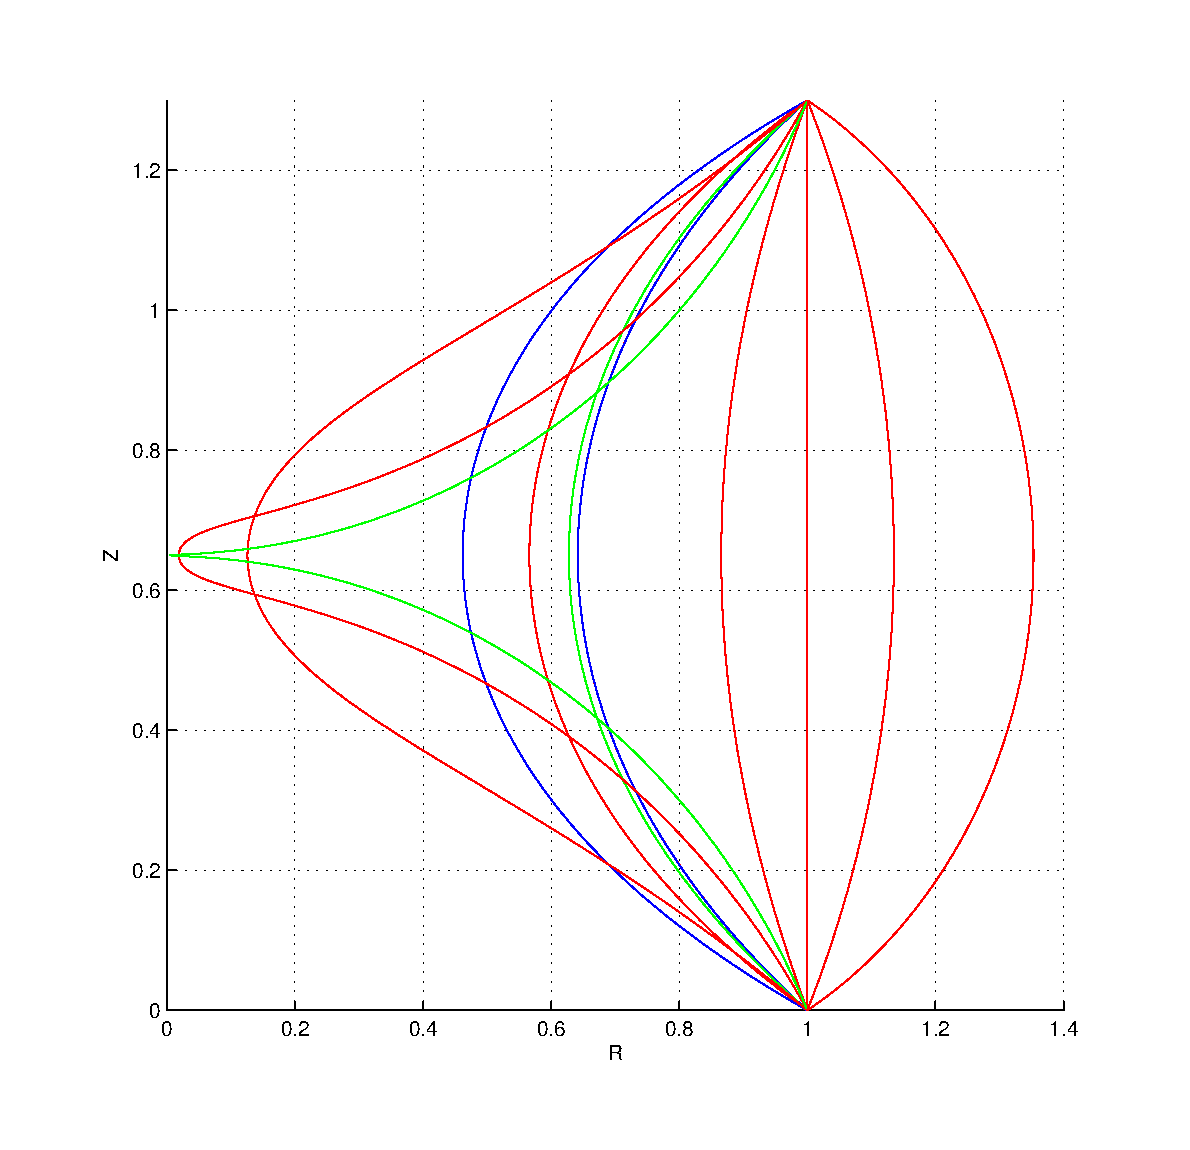
\includegraphics[width=.4\linewidth]{ShapeBridges_L1_3.eps}
\\
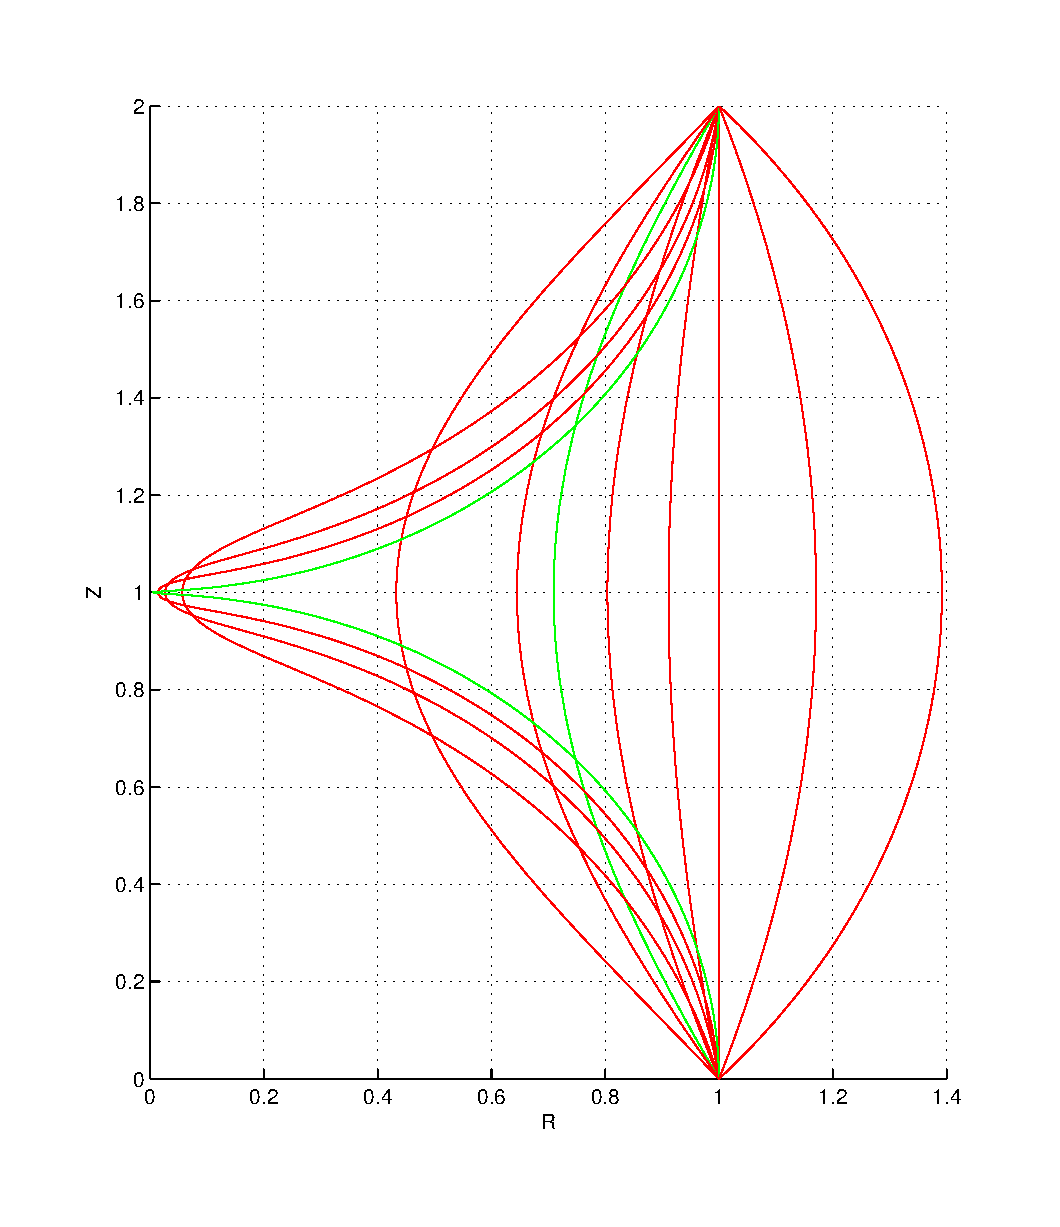
\includegraphics[width=.4\linewidth]{ShapeBridges_L2.eps}
\end{tabular}
}
\vcenteredhbox{
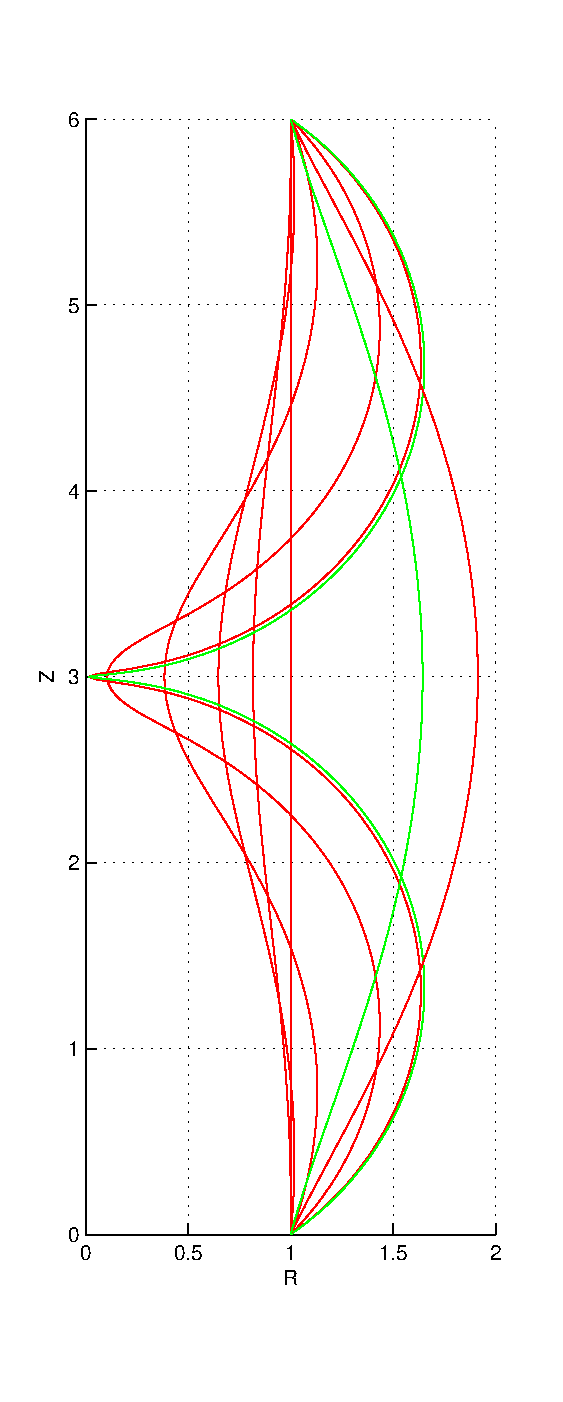
\includegraphics[width=.4\linewidth]{ShapeBridges_L6.eps}
}
\caption{A few equilibrium shapes for liquid bridges, for $L/a= 1.3$, $2$ and $6$.
The green shapes correspond to the limit case where the bridge becomes two touching spherical portions, and to the configuration with the same volume. }
\end{figure}




